\documentclass{../source/Experiment}

\major{信息工程}
\name{姚桂涛}
\title{LabVIEW 介绍}
\stuid{3190102932}
\college{信息与电子工程学院}
\date{\today}
\lab{——}
\course{通信原理实验}
\instructor{金向东、龚淑君}
\grades{}
\expname{LabVIEW 介绍}
\exptype{仿真+验证}
\partner{叶慷鹏}
\begin{document}
    \makecover
    \makeheader
    \section{实验目的}
    (1) 熟悉LabVIEW 通信设计套件

    (2) 会使用While/For 循环处理数据

    (3) 熟悉多种数据类型

    (4) 会使用数组,访问和处理元素

    \section{实验内容}
        \subsection{While循环}
        While 循环是一个控制流语句,用于重复执行一个函数,直到满足给定的条件终端。条
        件终端定义循环结束的时间。条件终端有两种设置:如果为True 则继续和如果为True 则停
        止。如果设置为True 继续,则仅当布尔控件返回True 时才进行循环。如果设置为True 则
        停止,布尔值为True 时,循环将中止。默认情况下,条件终端是“True 则停止”。
        \subsubsection{While循环示例}
        使用while 循环,产生一组0 到10 之间的随机整数,当产生的数与用户给定的数值匹配是,停止产生随机数。
        \subsubsection{问题1}
        \begin{enumerate}
            \item 完成以上示例
            \item 给while 循环增加一些延时(比如1 秒钟),以便能观察到数据的变化。
            \item 增加一个布尔指示器,当随机数大于5 时打开,小于或等于5 时关闭。
            \item 增加一个输出端显示循环的次数。
        \end{enumerate}

        (1) 示例完成如下:

        \begin{figure}[H]
            \centering
            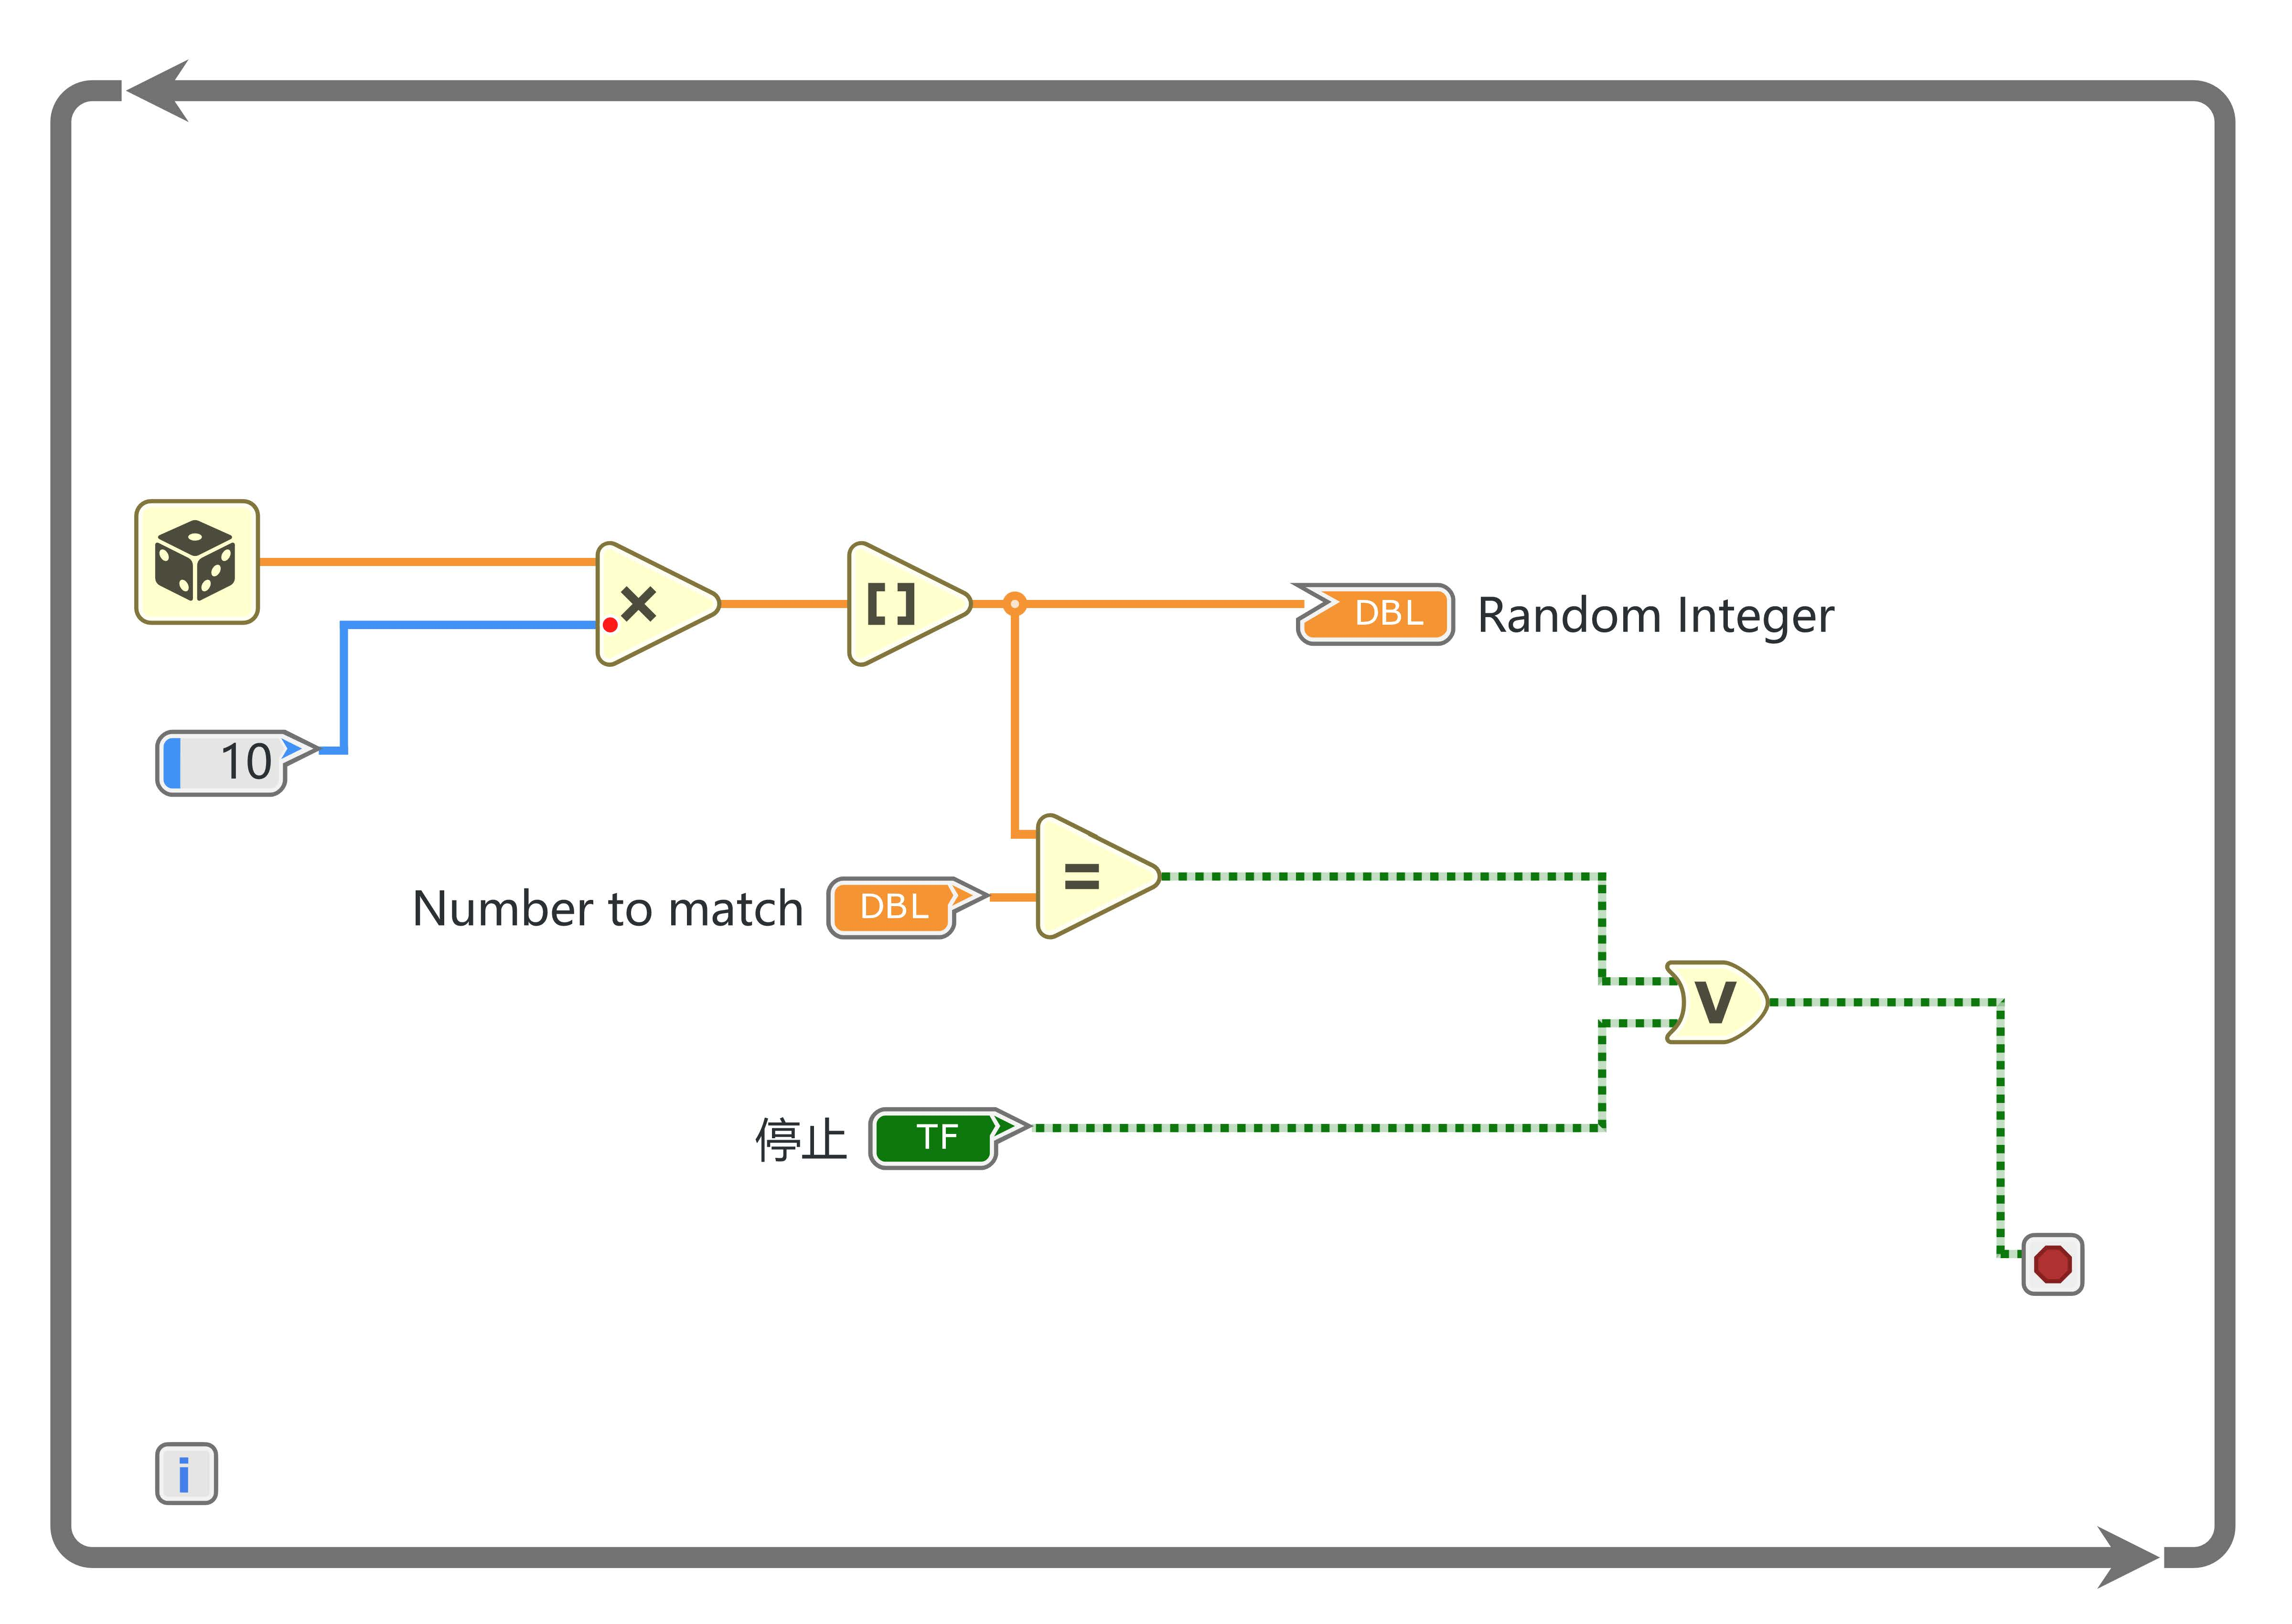
\includegraphics[width = 0.6\textwidth]{lab8/lab1-a.jpg}
            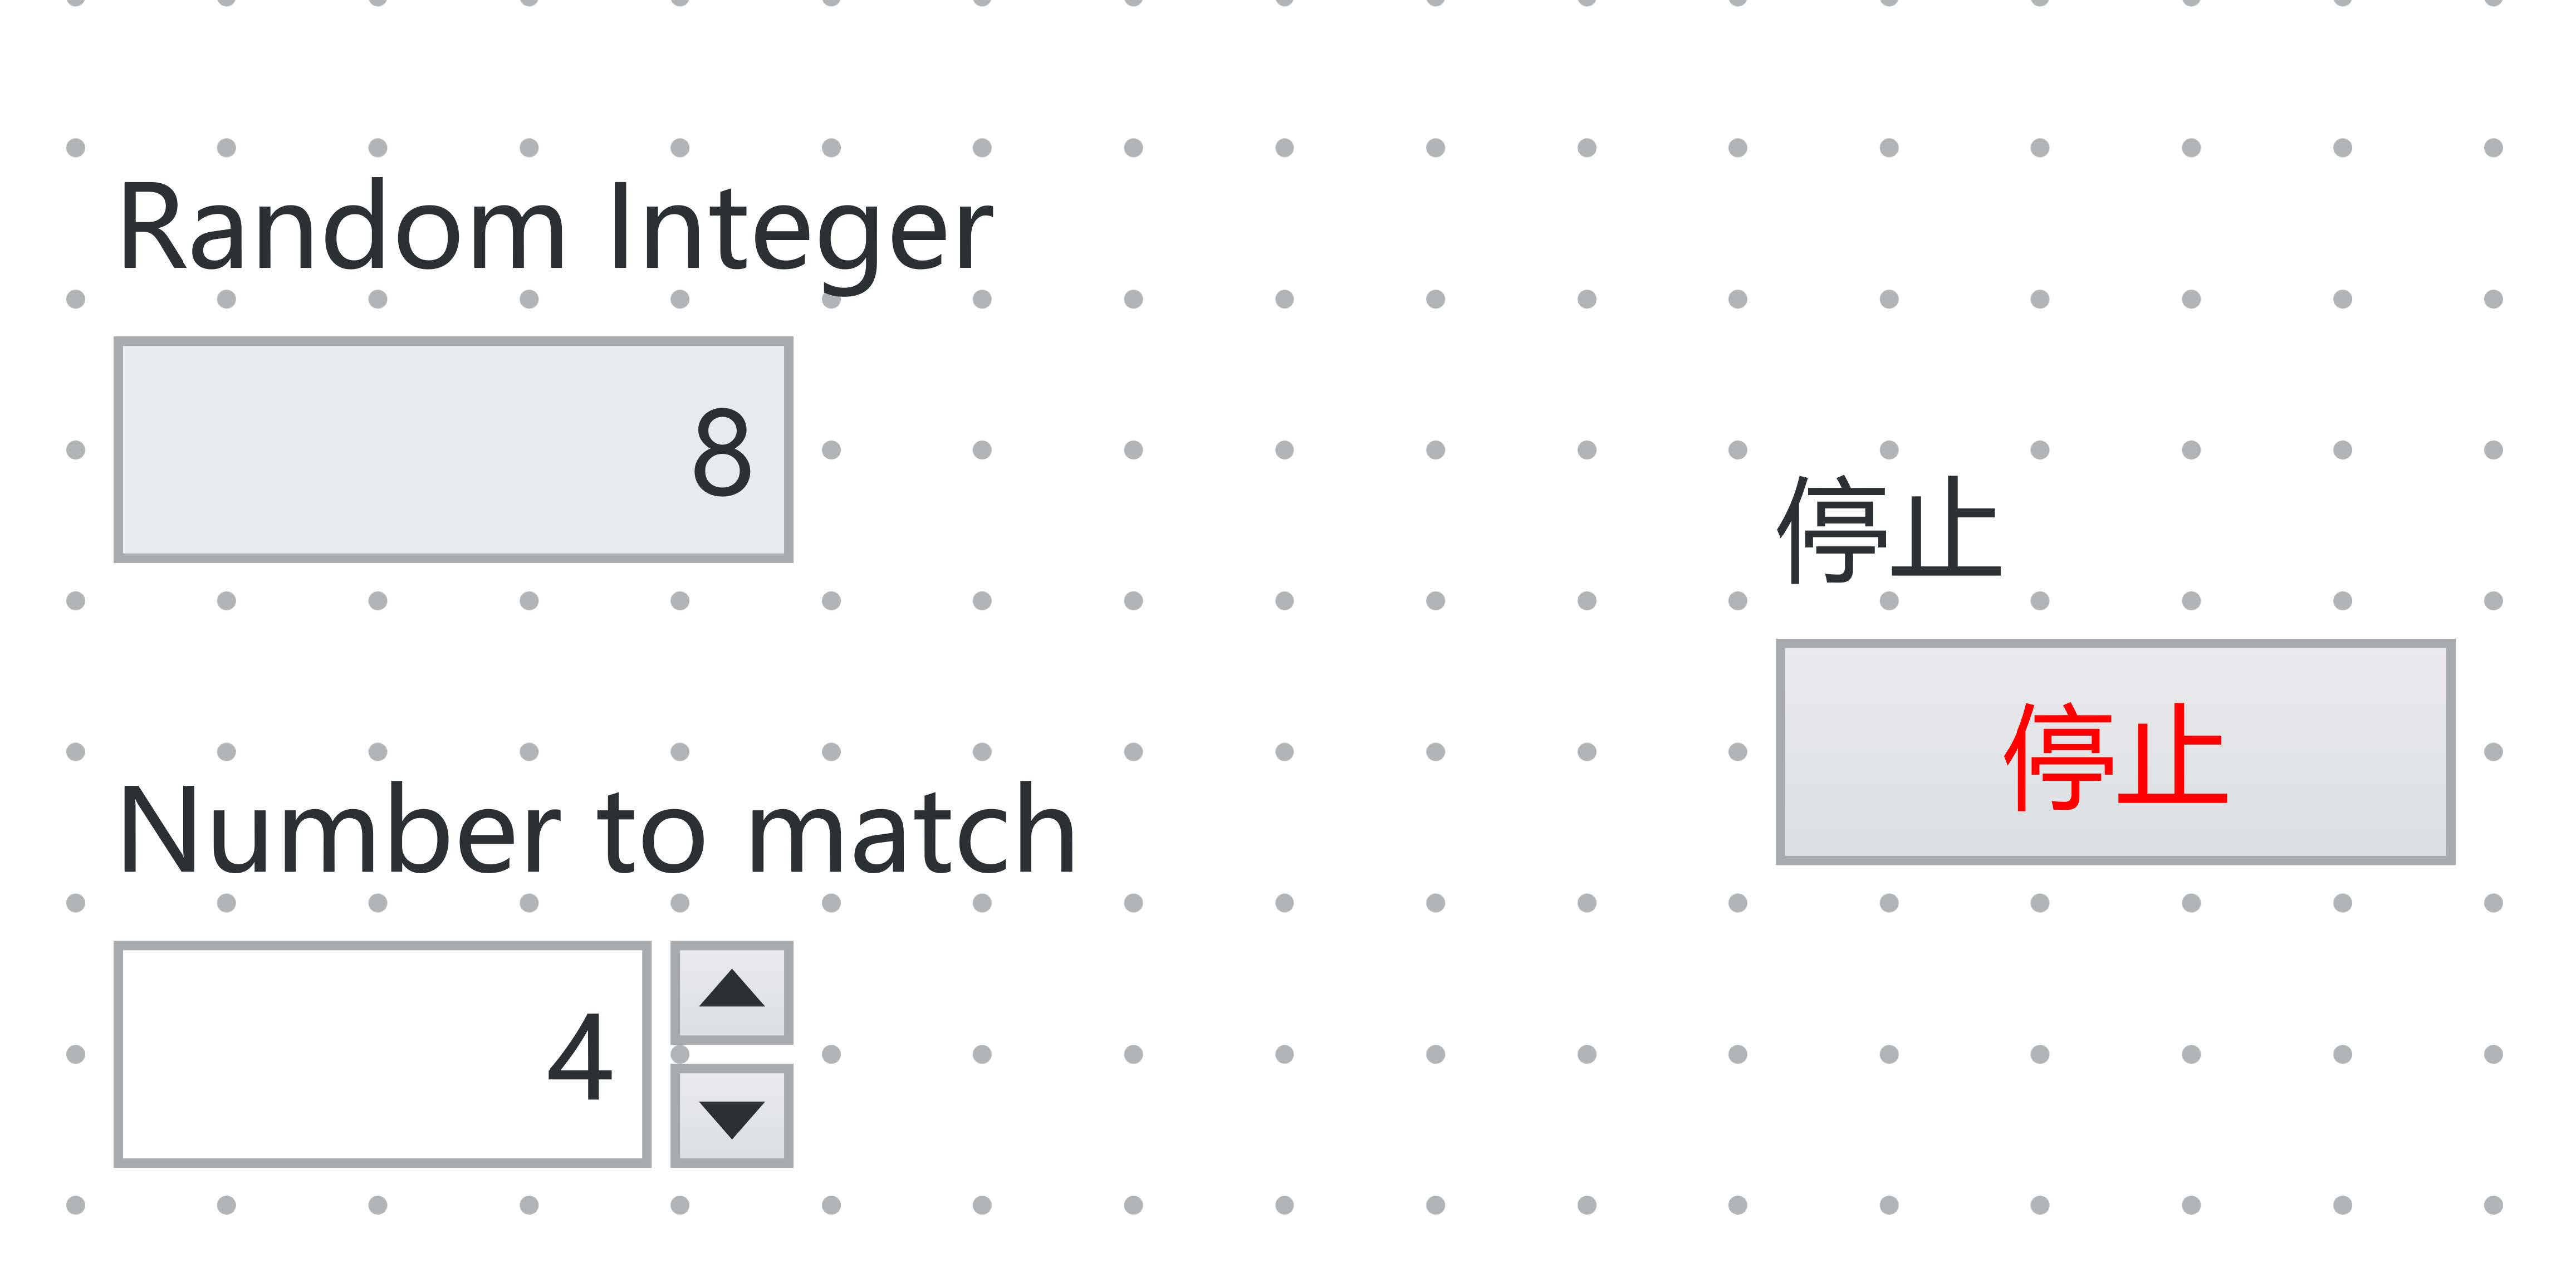
\includegraphics[width = 0.38\textwidth]{lab8/lab1-b.jpg}
            \caption{完成示例1}
        \end{figure}

        (2)、(3)、(4) 改进如下:
        \begin{figure}[H]
            \centering
            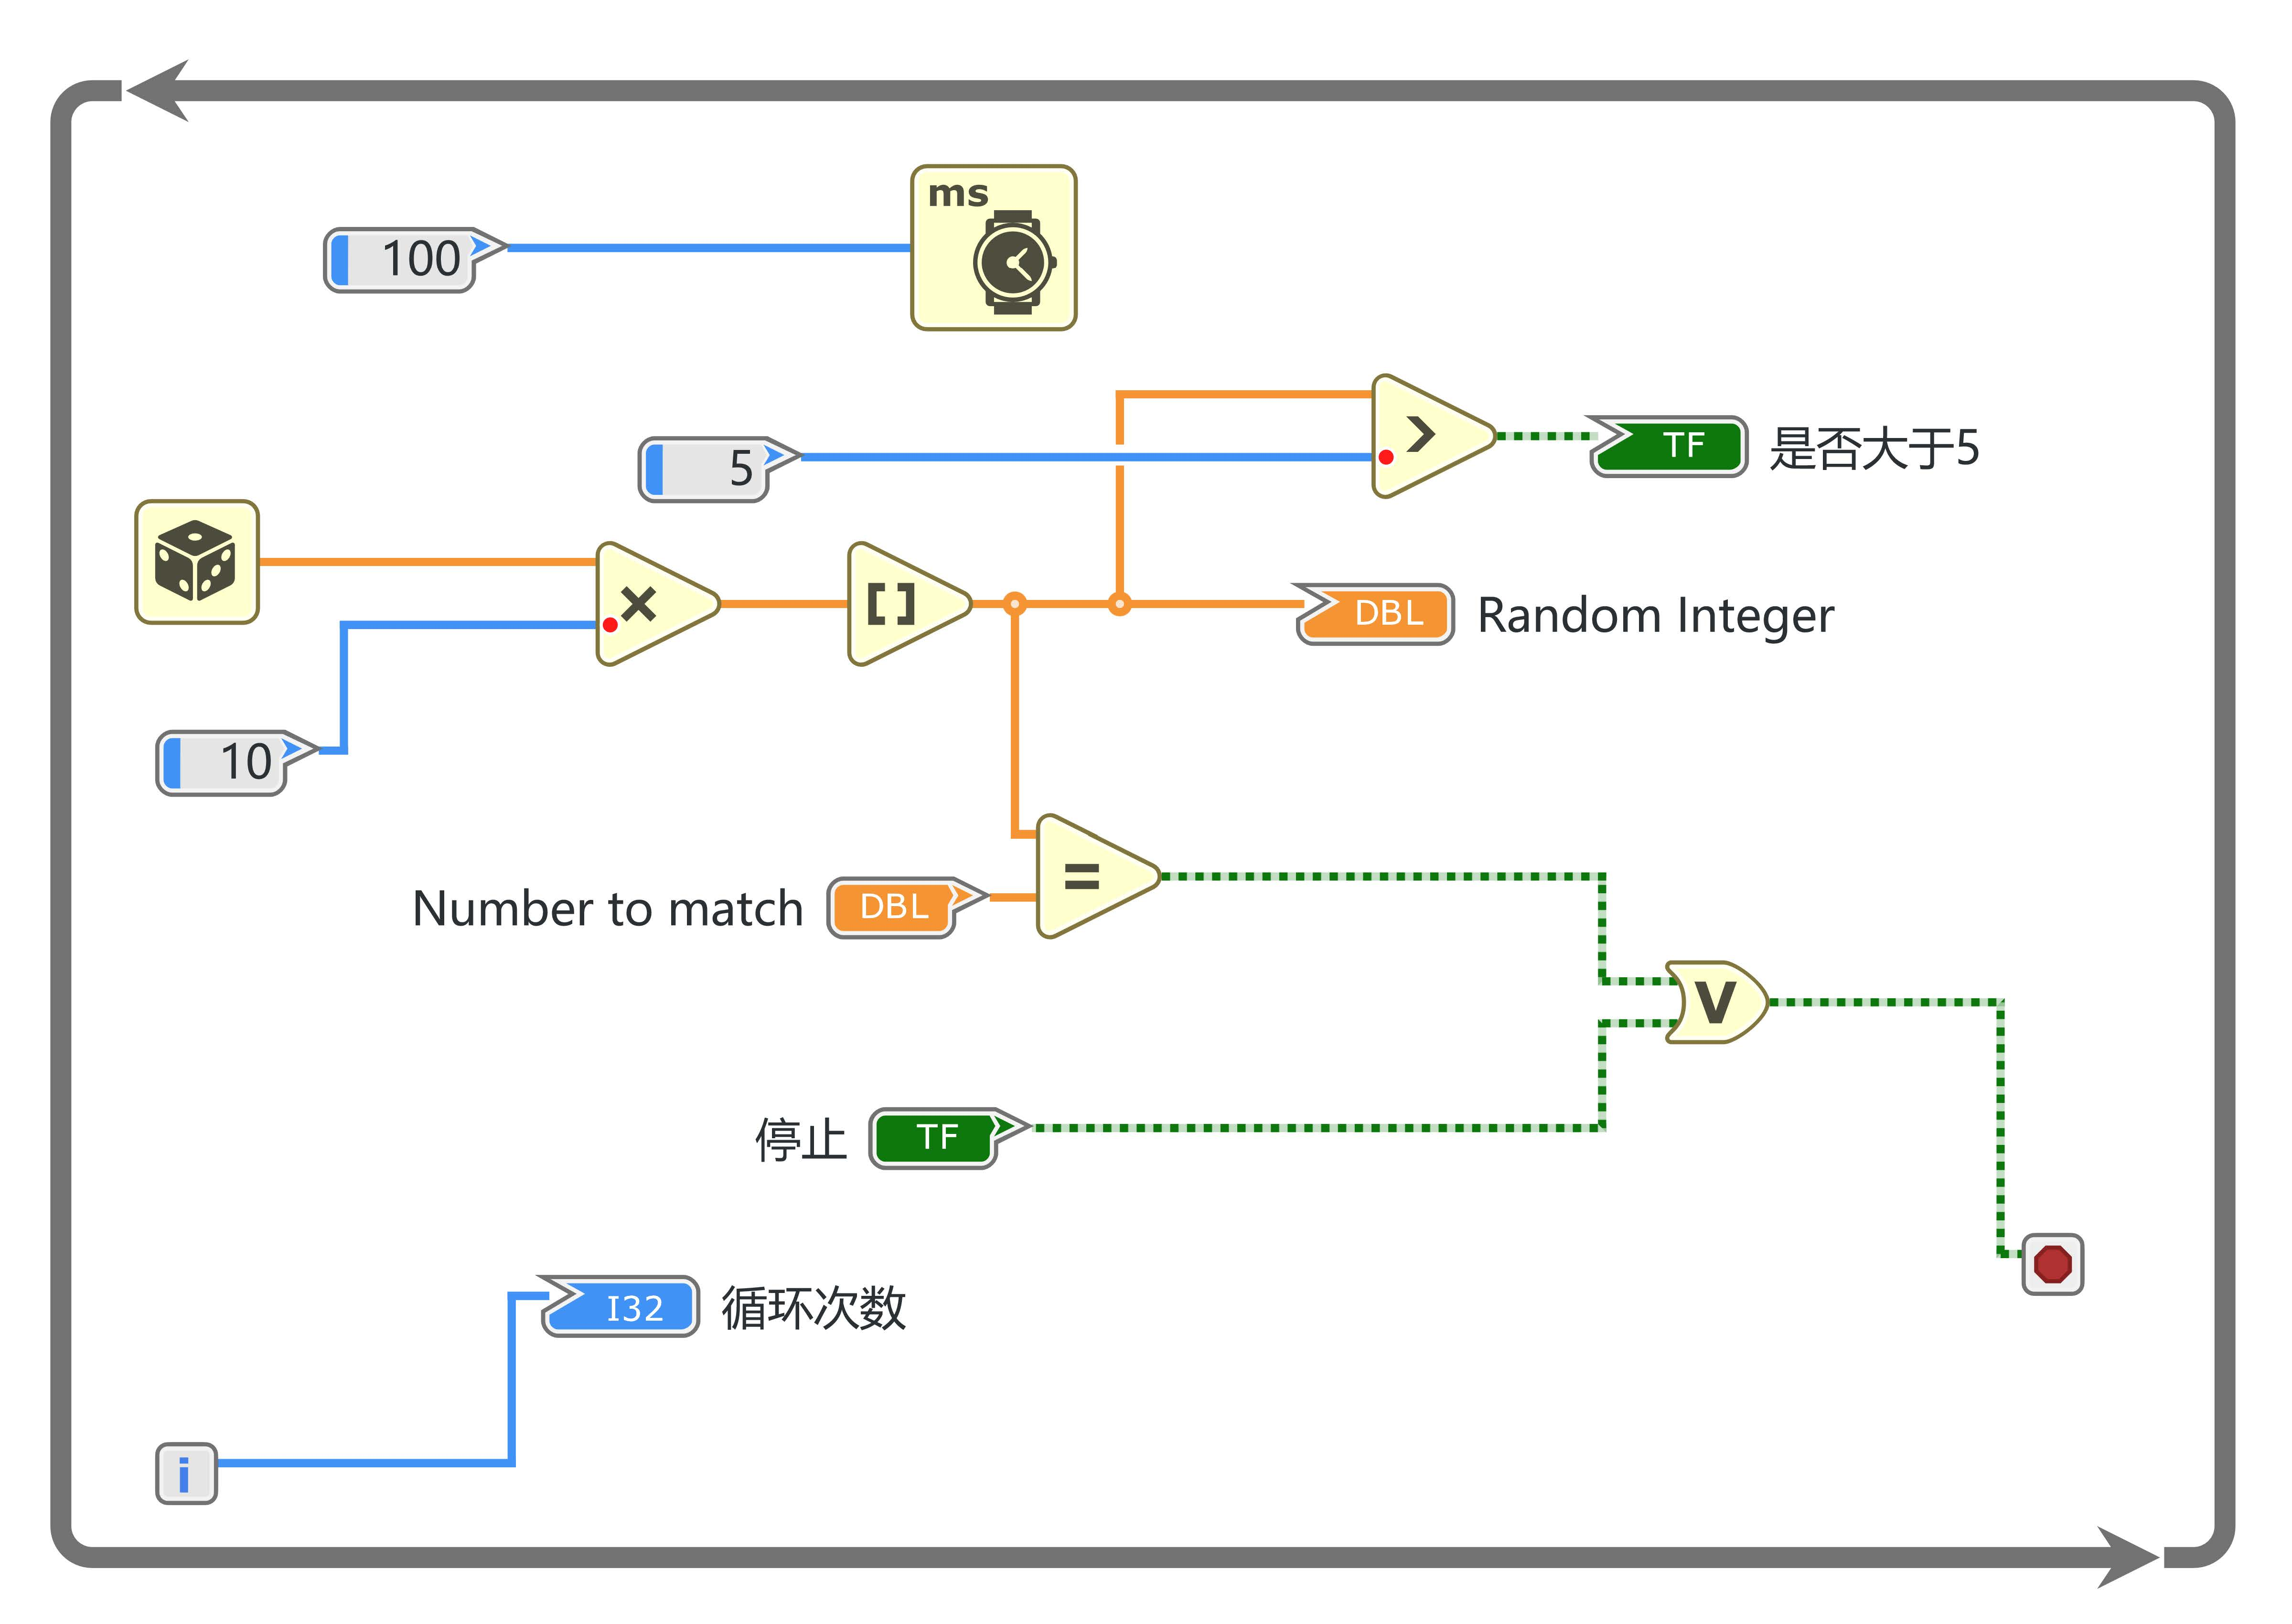
\includegraphics[width = 0.6\textwidth]{lab8/lab1改进-a.jpg}
            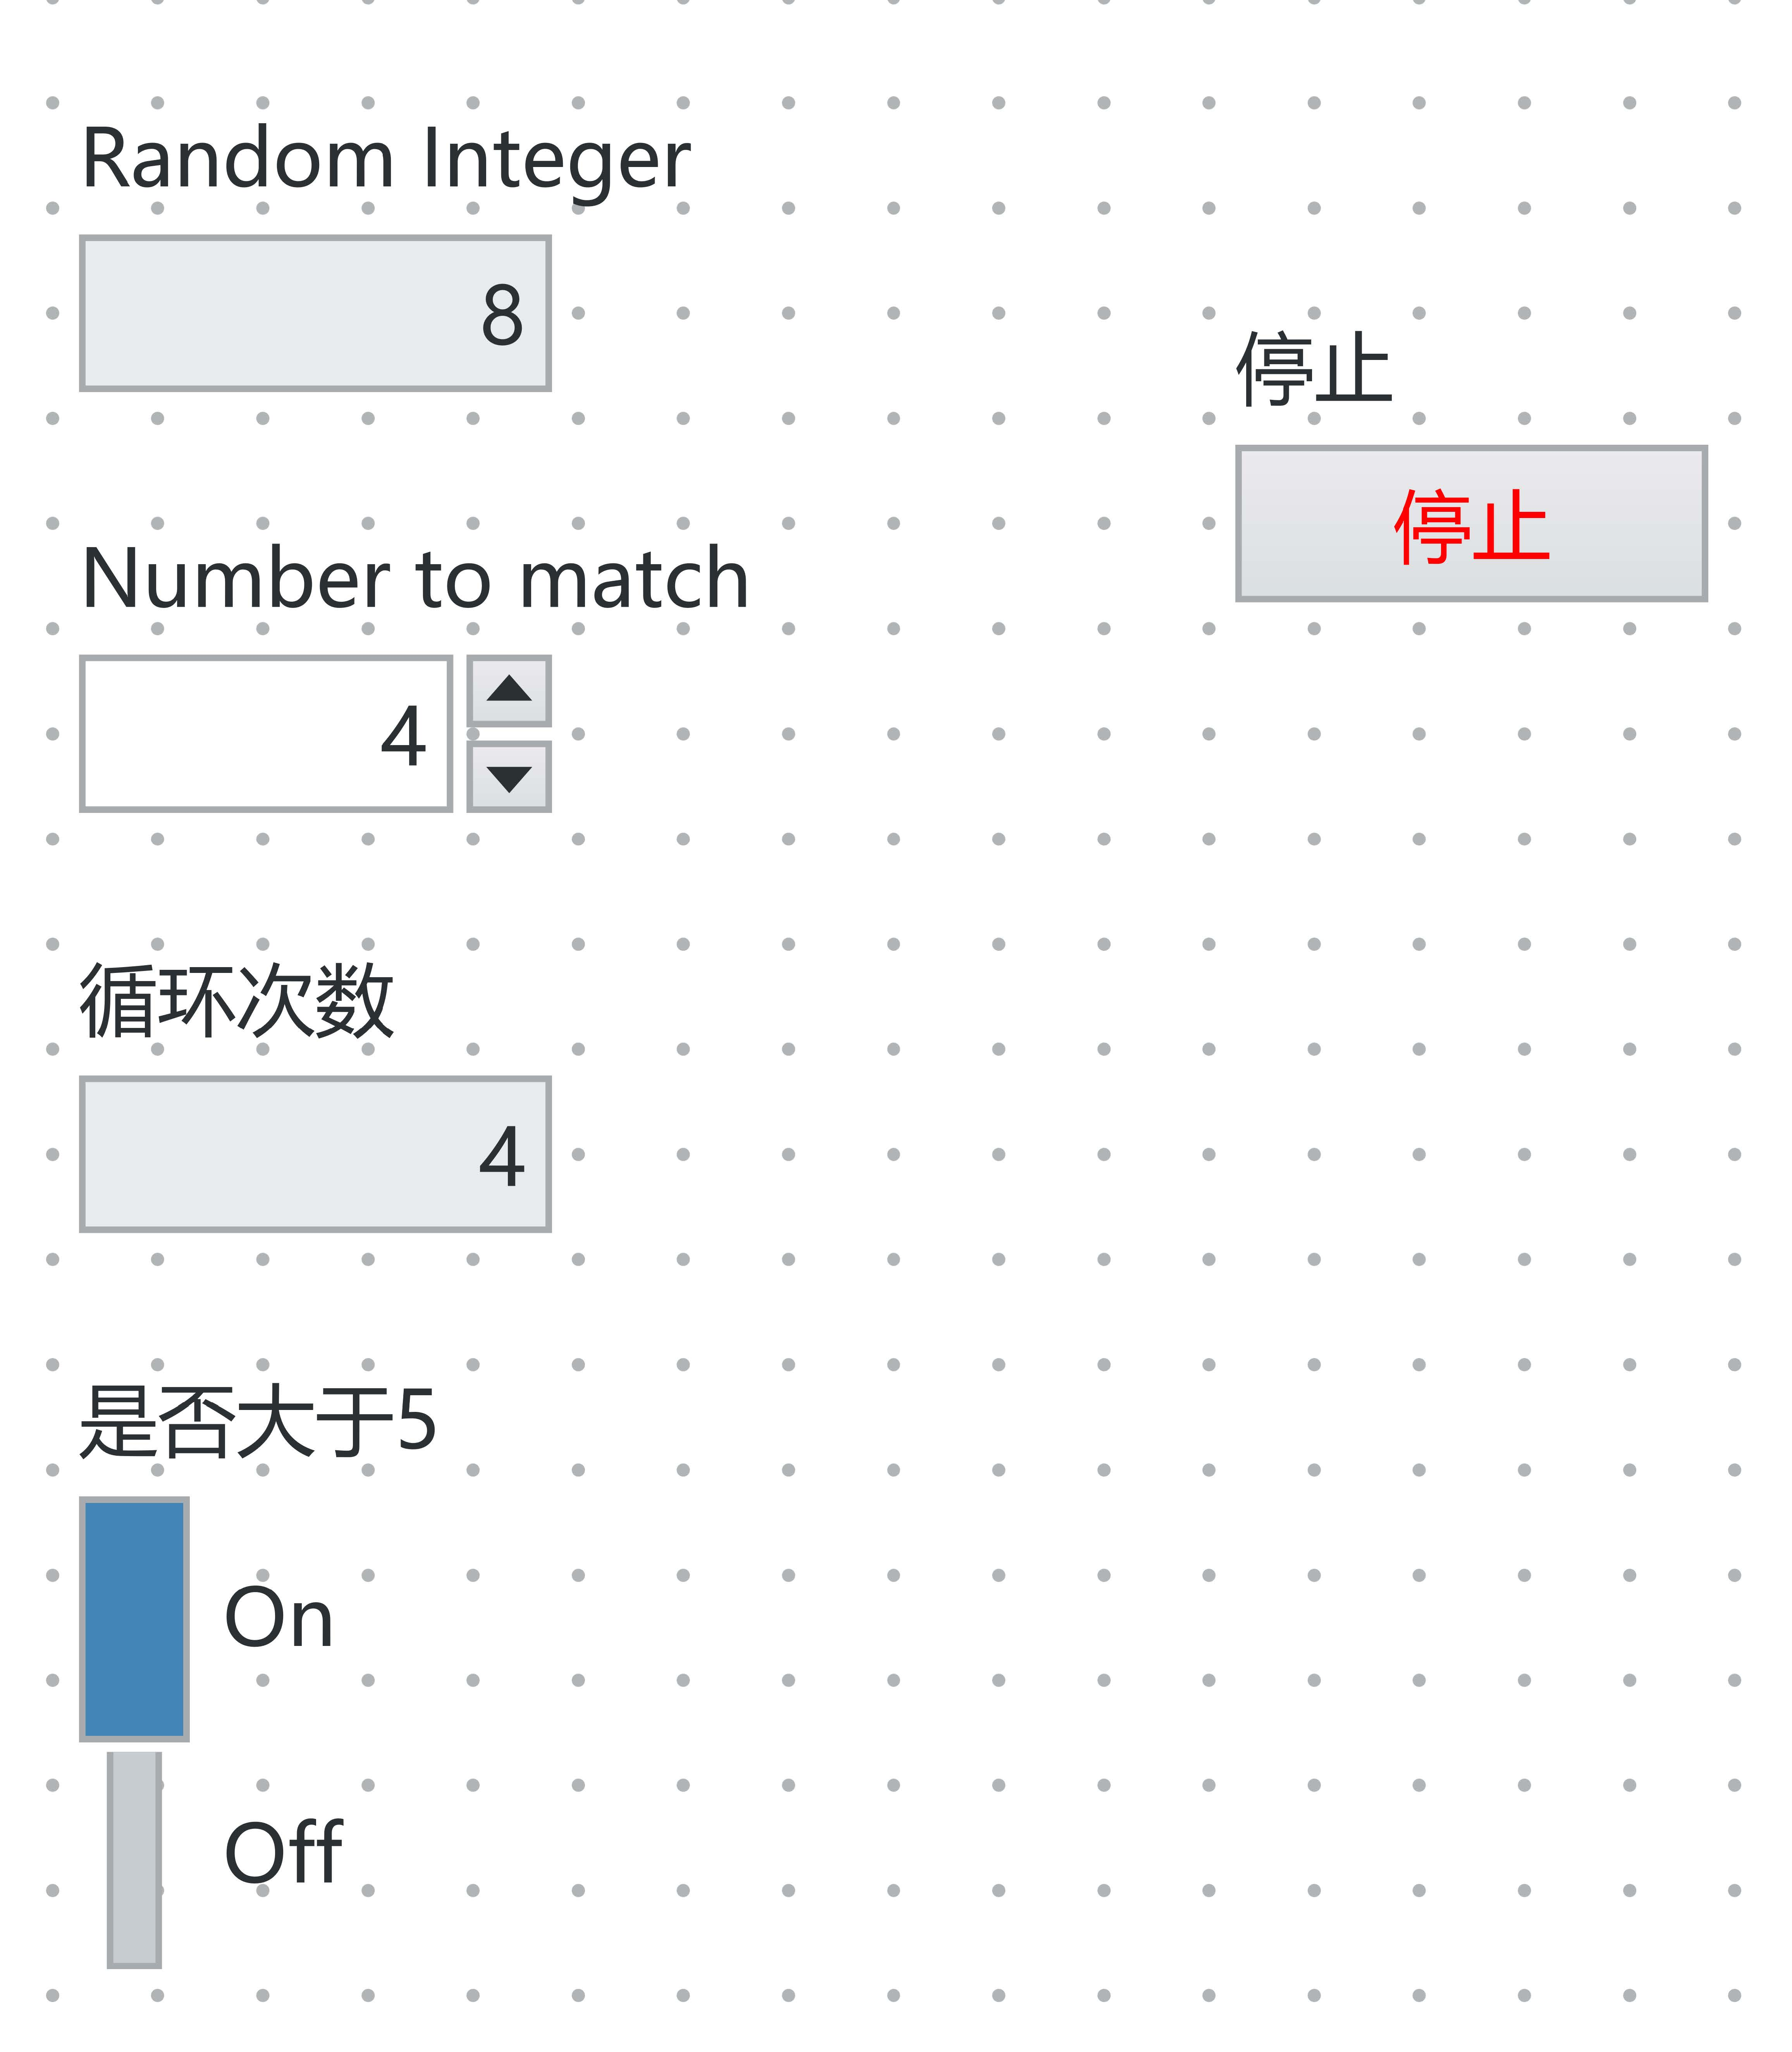
\includegraphics[width = 0.38\textwidth]{lab8/lab1改进-b.jpg}
            \caption{示例1改进}
        \end{figure}
        \subsection{数据类型}
        在LabVIEW 中,每一个对象和连线都跟数据类型有关系。LabVIEW 支持很多数据类型,它们由不同的颜色、形状区分。部分数据类型如下图所示:
        \begin{figure}
            \centering
            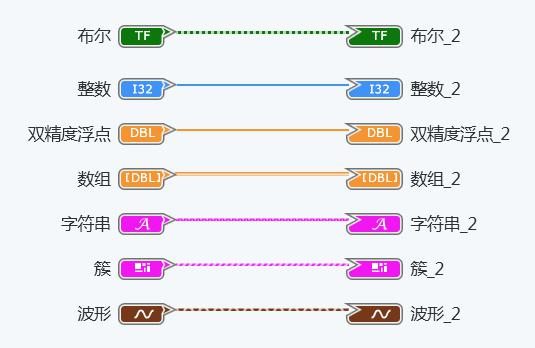
\includegraphics[width = 0.5\textwidth]{lab8/fig1.jpg}
        \end{figure}
        \subsubsection{数据类型示例}
        下面列举簇数据类型的使用:接收一串字符串,将其反转;对给定的数组元素数值增加偏置量。
        \subsubsection{问题2}
        \begin{enumerate}
            \item 完成上面的示例,在实验报告中提供程序框图和前面板运行结果。
            \item 是否能将一个整型控制输入与双精度类型显示输出相连?整型输入能否与字符串输出
            相连?如果不可以,需要使用什么模块进行类型转换?
        \end{enumerate}
        (1)  示例完成如下:

        \begin{figure}[H]
            \centering
            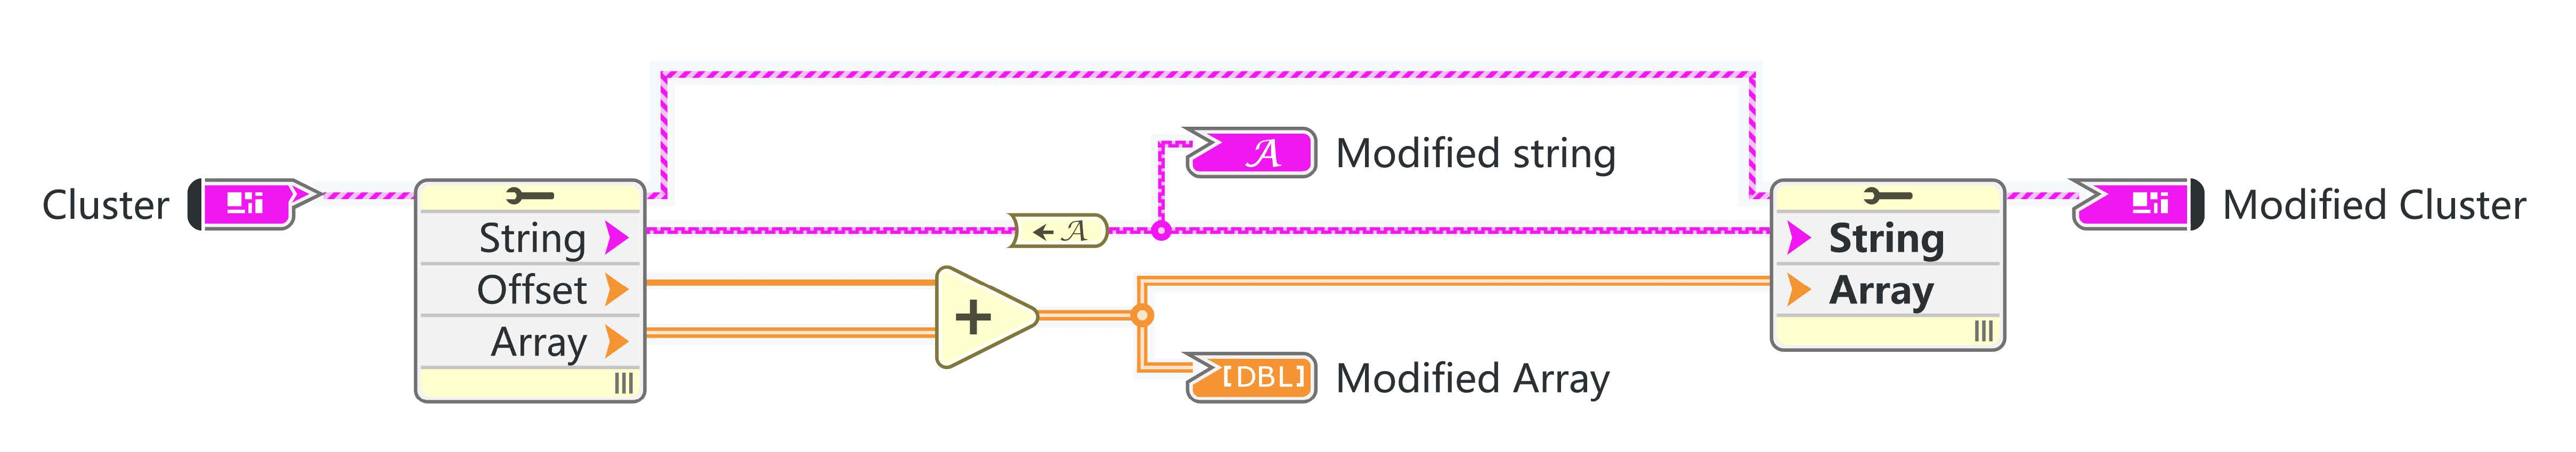
\includegraphics[width = 0.8\textwidth]{lab8/lab1-3-a.jpg}
            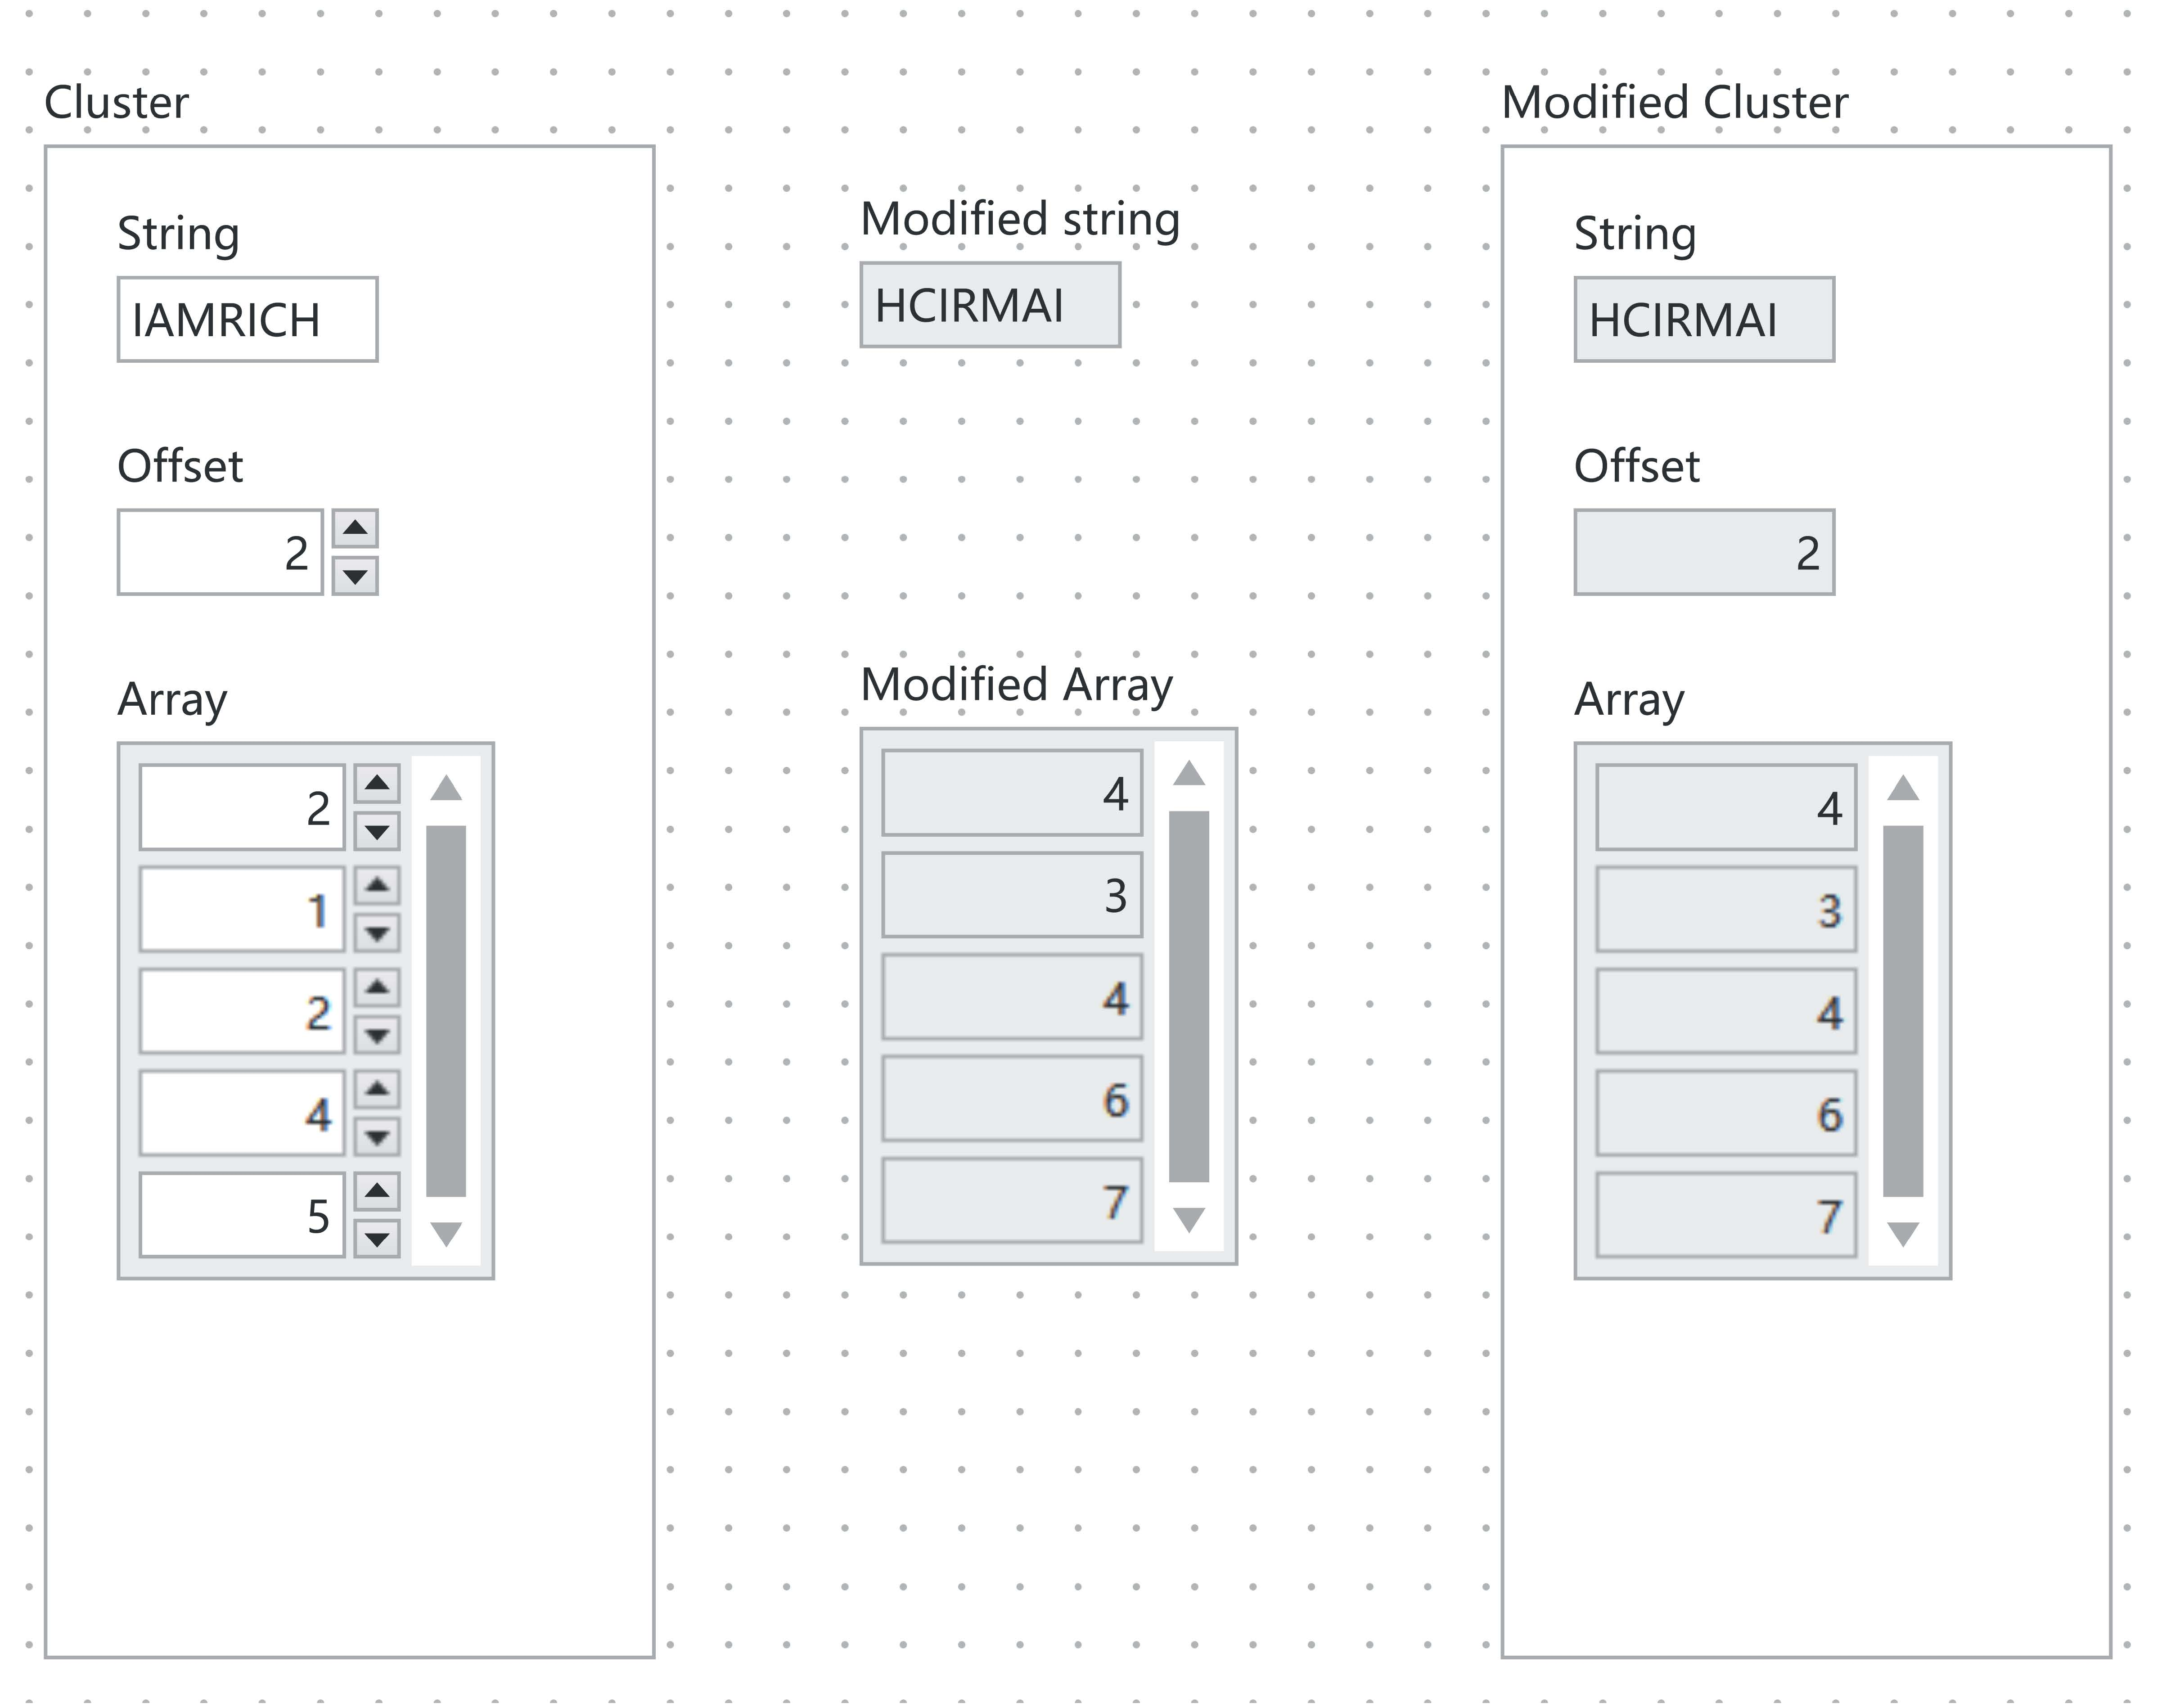
\includegraphics[width = 0.5\textwidth]{lab8/lab1-3-b.jpg}
            \caption{完成示例2}
        \end{figure}

        (2)  可以将一个整型控制输入与双精度类型显示输出相连,软件会自动进行数据类型转换;但是不能将整型输入与字符串输出相连,需要用一个数值至十进制数字符串转换模块进行类型转换。

        \subsection{数组}
        数值中的元素都是相同类型的数据,可以是数值、布尔、路径、字符串、波形和簇。当
        处理一批类似数据或作重复计算时,可以考虑使用数组。存储波形数据或循环中产生的数据
        时,使用数组是一个理想选择。
        \subsubsection{数组示例}
        给定一个数值数组,找出其中的最大元素。
        \subsubsection{问题3}
        \begin{enumerate}
            \item 完成上面的示例,在实验报告中提供程序框图和前面板运行结果。
            \item 将数组元素最大值改为0,再次运行程序,还能找到最大值吗?更改例程,使得每运一次程序都能找到最大值。
            \item 在问题2 的基础上,更改程序框图,能够得到最大值的索引值(在数组中的位置)。
            \item 完成以下VI:产生两个数值范围在-0.5 到0.5 之间的随机数,比较这两个随机数值的大
            小,如果第一个数比第二个数大,Team A 得分;如果第二个数比第一个数大,Team B
            得分。当其中一个队得分达到50 时,程序停止运行。显示最终的两个随机数、循环的
            次数、Team A 和Team B 的得分以及哪一对赢。
        \end{enumerate}
        
        (1) 示例完成如下:

        \begin{figure}[H]
            \centering
            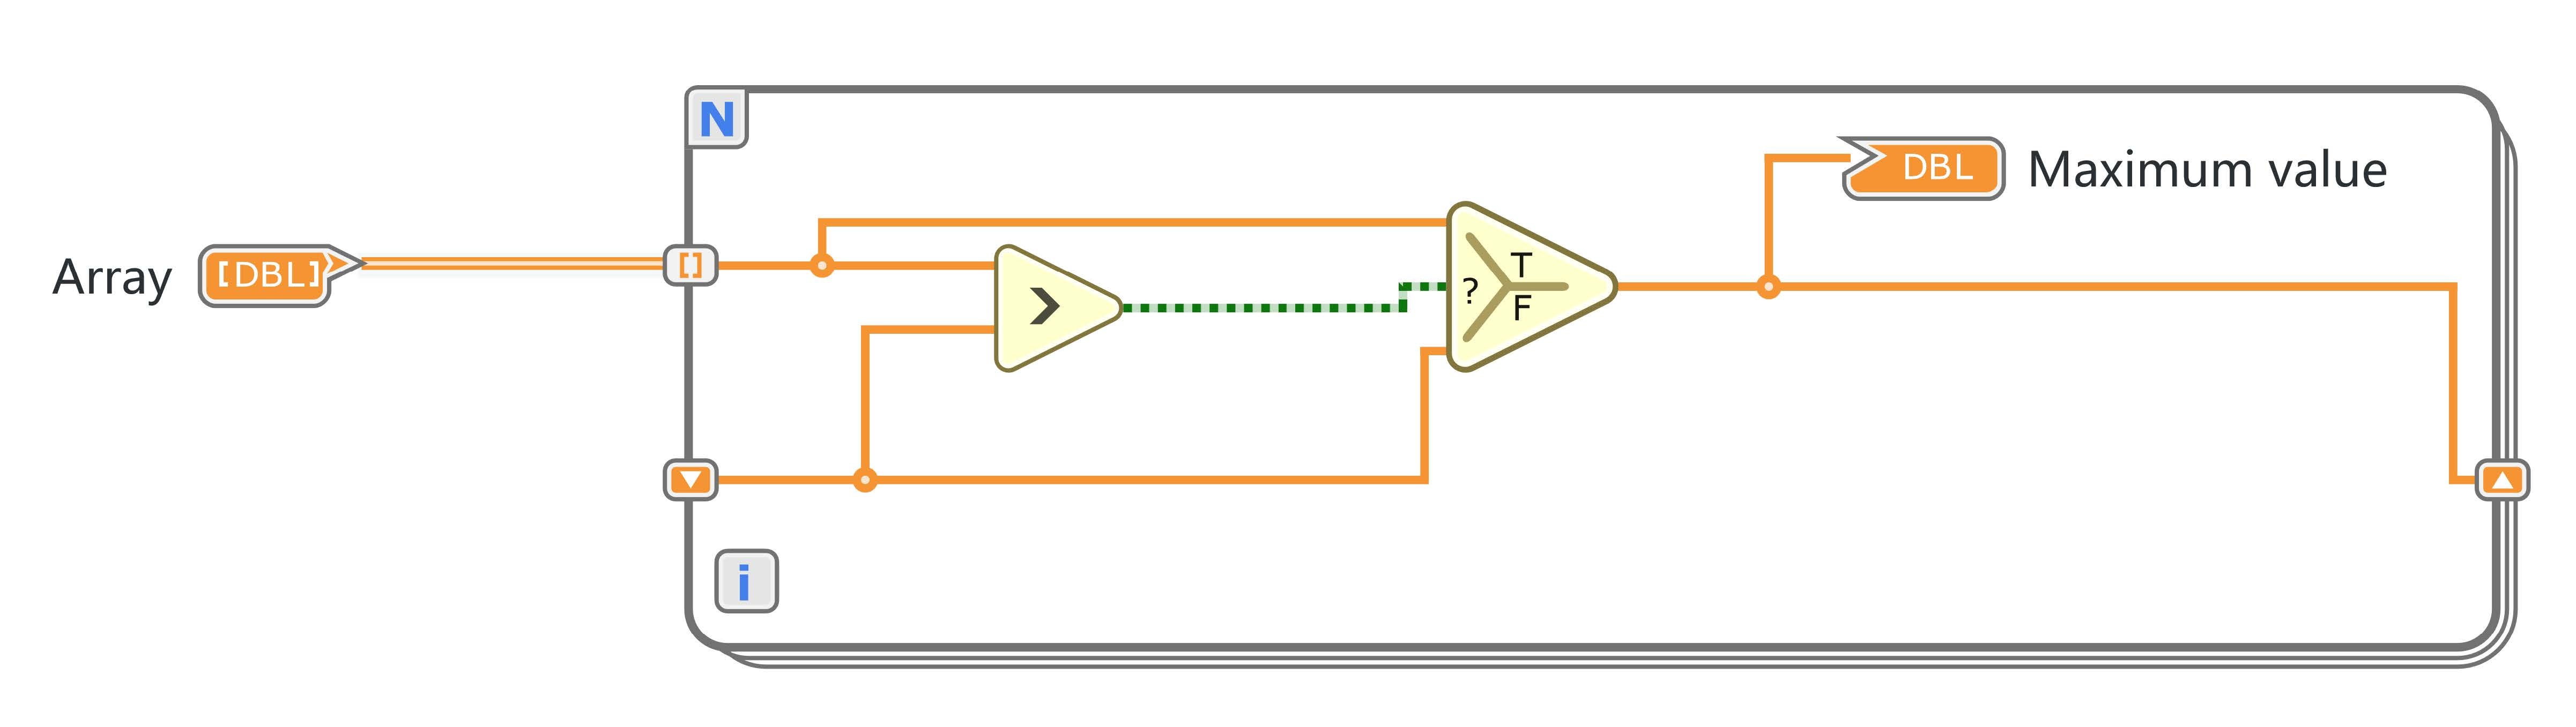
\includegraphics[width = 0.7\textwidth]{lab8/lab1-数组-a.jpg}
            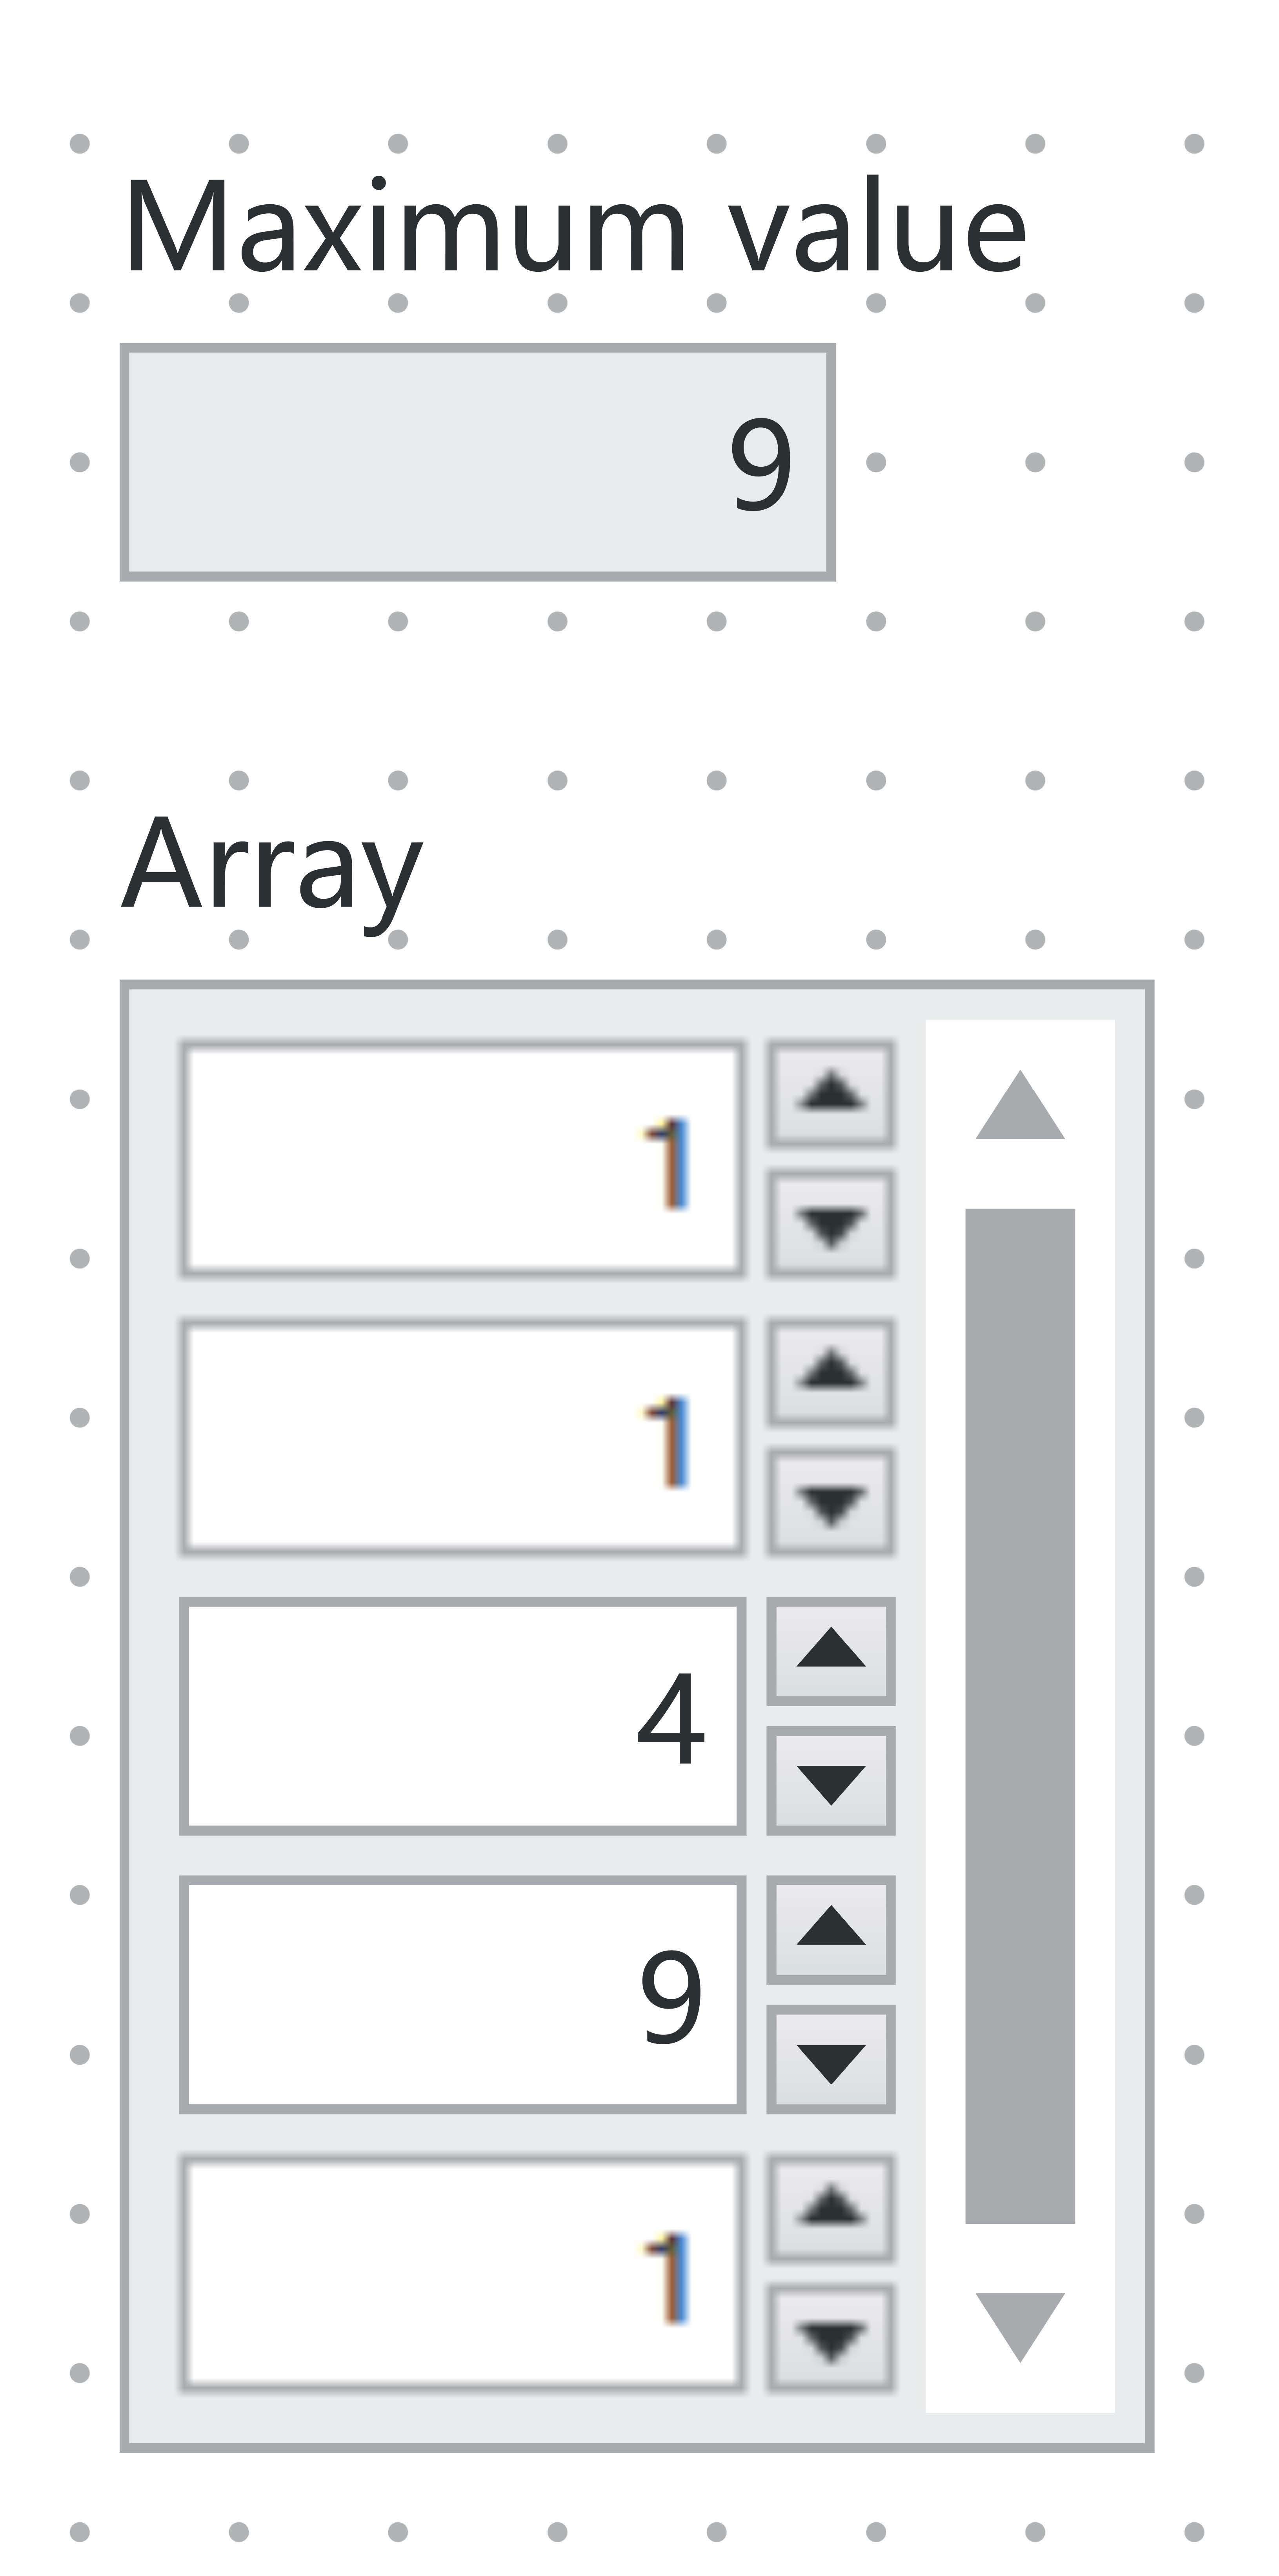
\includegraphics[width = 0.18\textwidth]{lab8/lab1-数组-b.jpg}
            \caption{完成示例}
        \end{figure}

        (2) 无法找到最大值,原因是示例中for循环的寄存器储存了上次的最大值,并且下次运行时会将输入值与其比较,所以如果新的最大值没有上次的最大值大,则无法找到新的最大值。

        (3) 得到最大值的索引值
    
        问题2、3的改进如下:
        \begin{figure}[H]
            \centering
            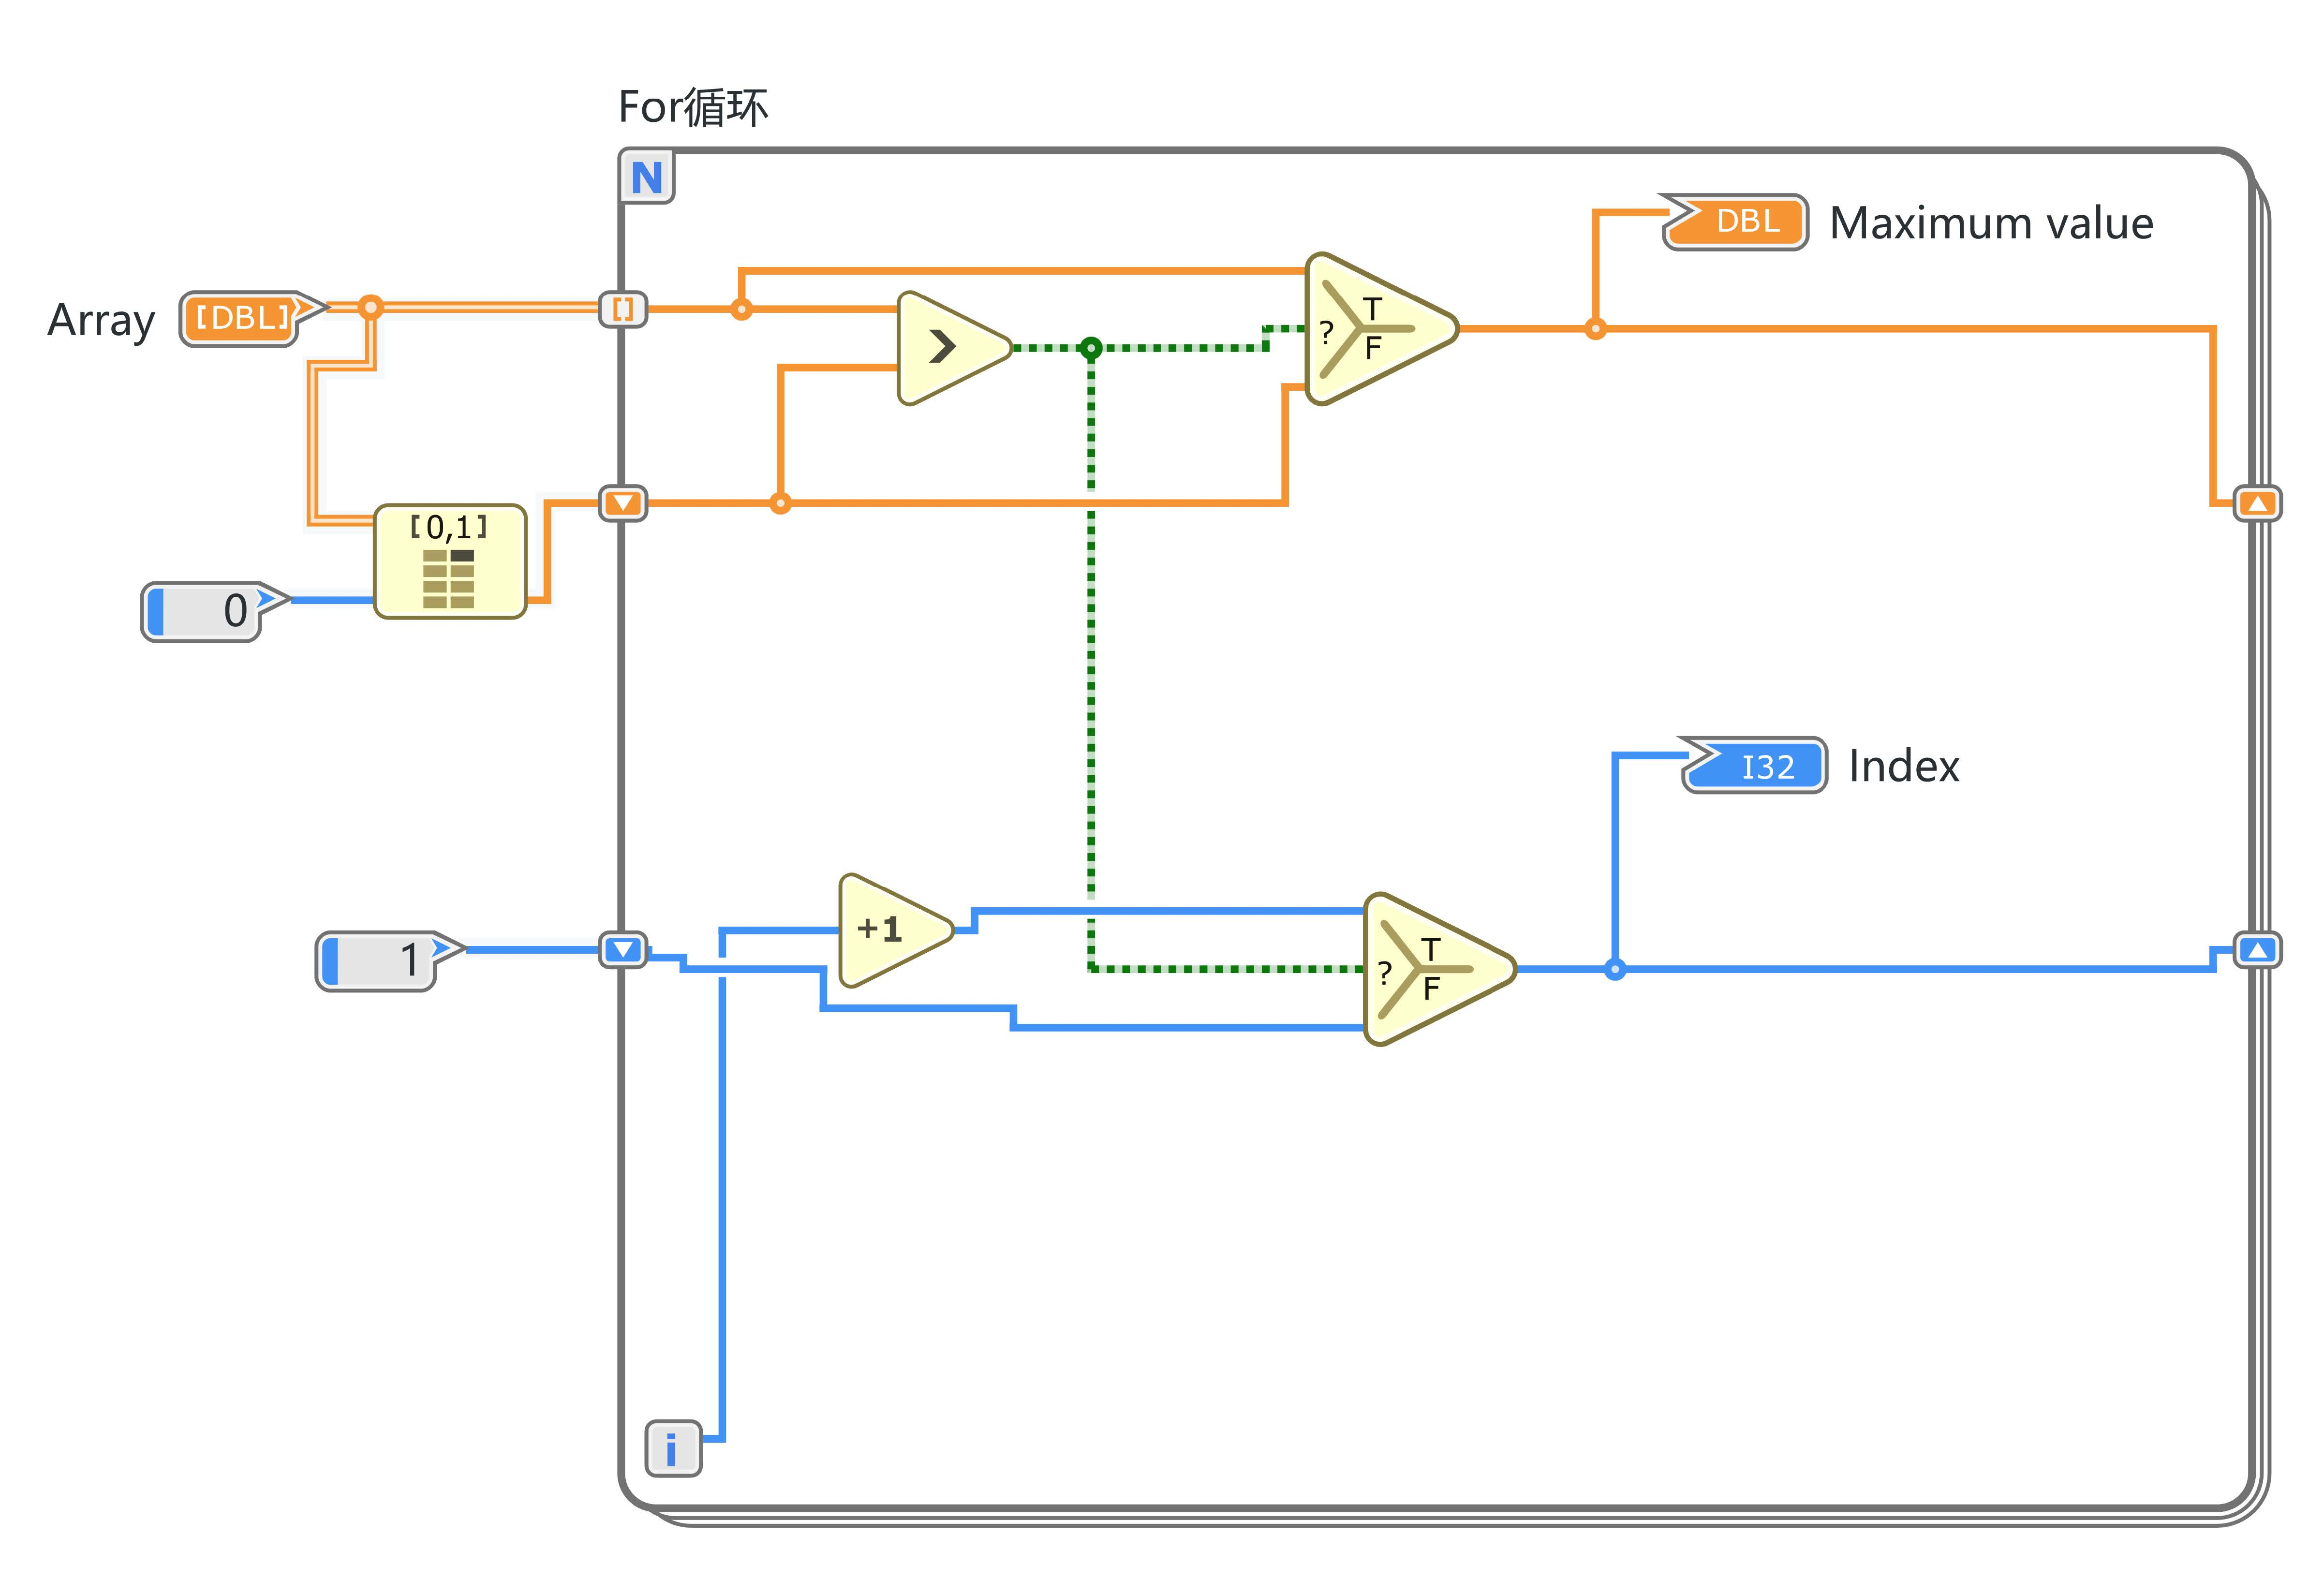
\includegraphics[width = 0.7\textwidth]{lab8/lab1-问题3-3-a.jpg}
            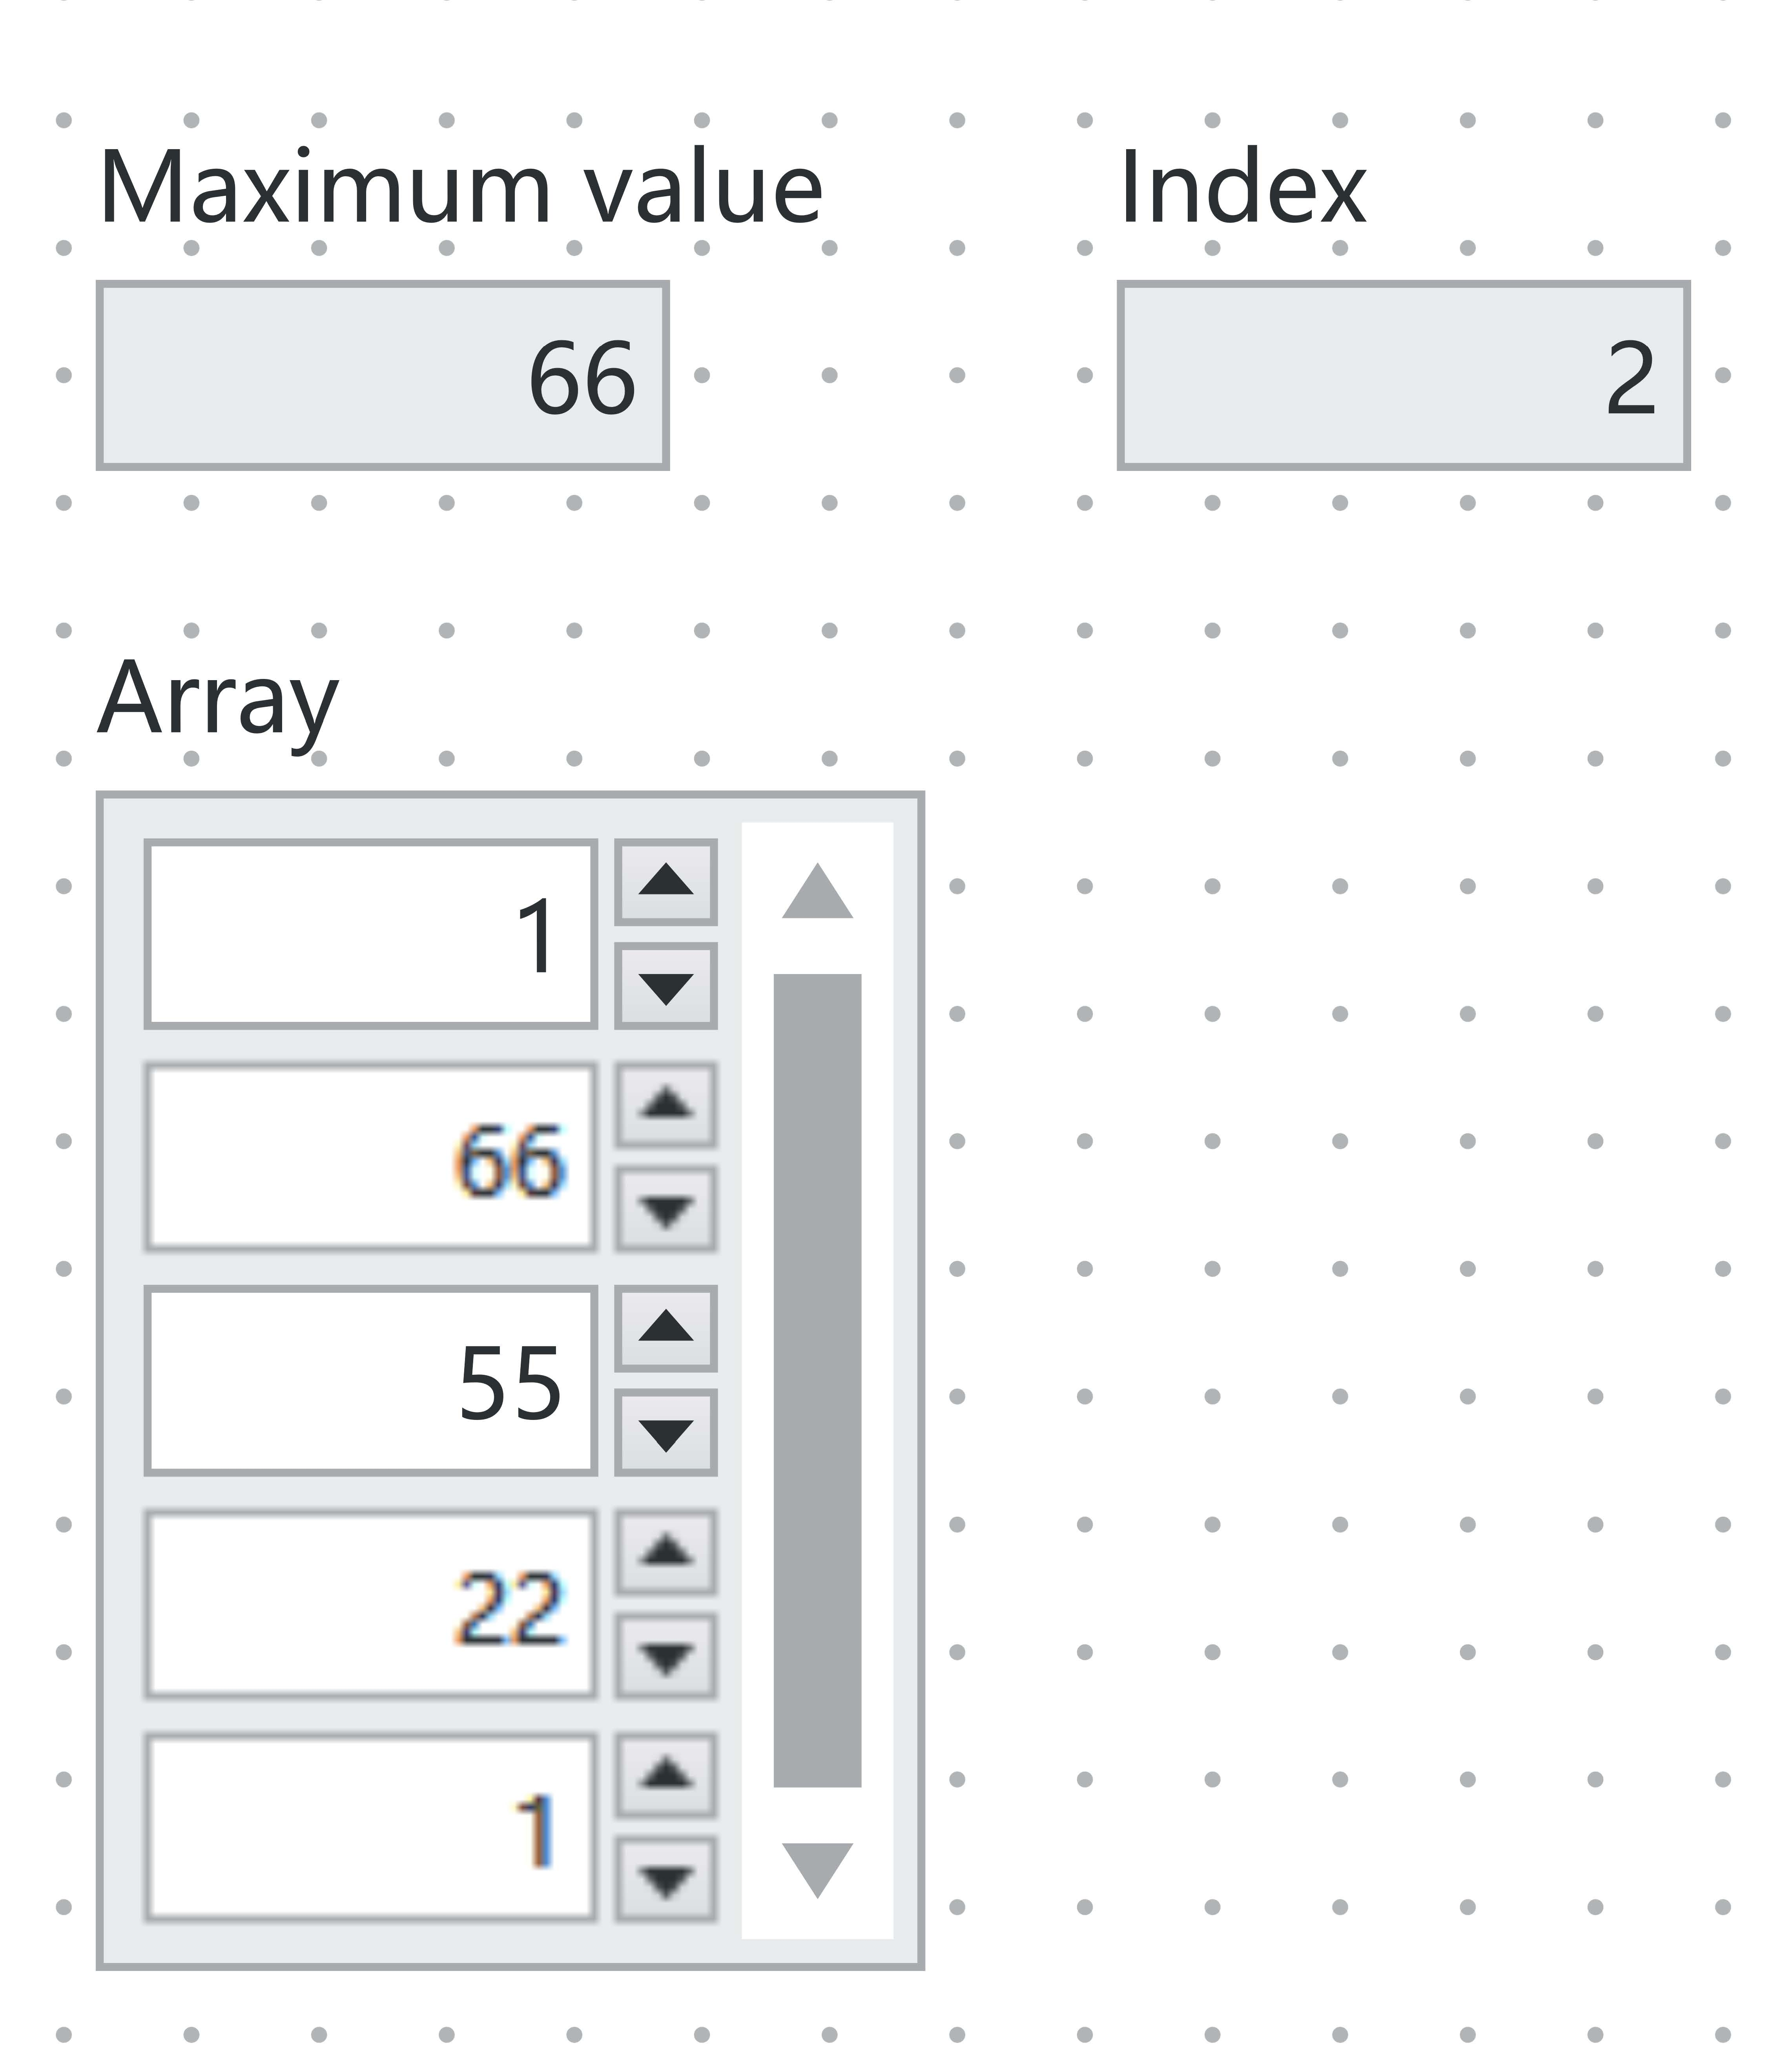
\includegraphics[width = 0.28\textwidth]{lab8/lab1-问题3-3-b.jpg}
            \caption{改进}
        \end{figure}

        (4)
        设计如下:
        
        \begin{figure}[H]
            \centering
            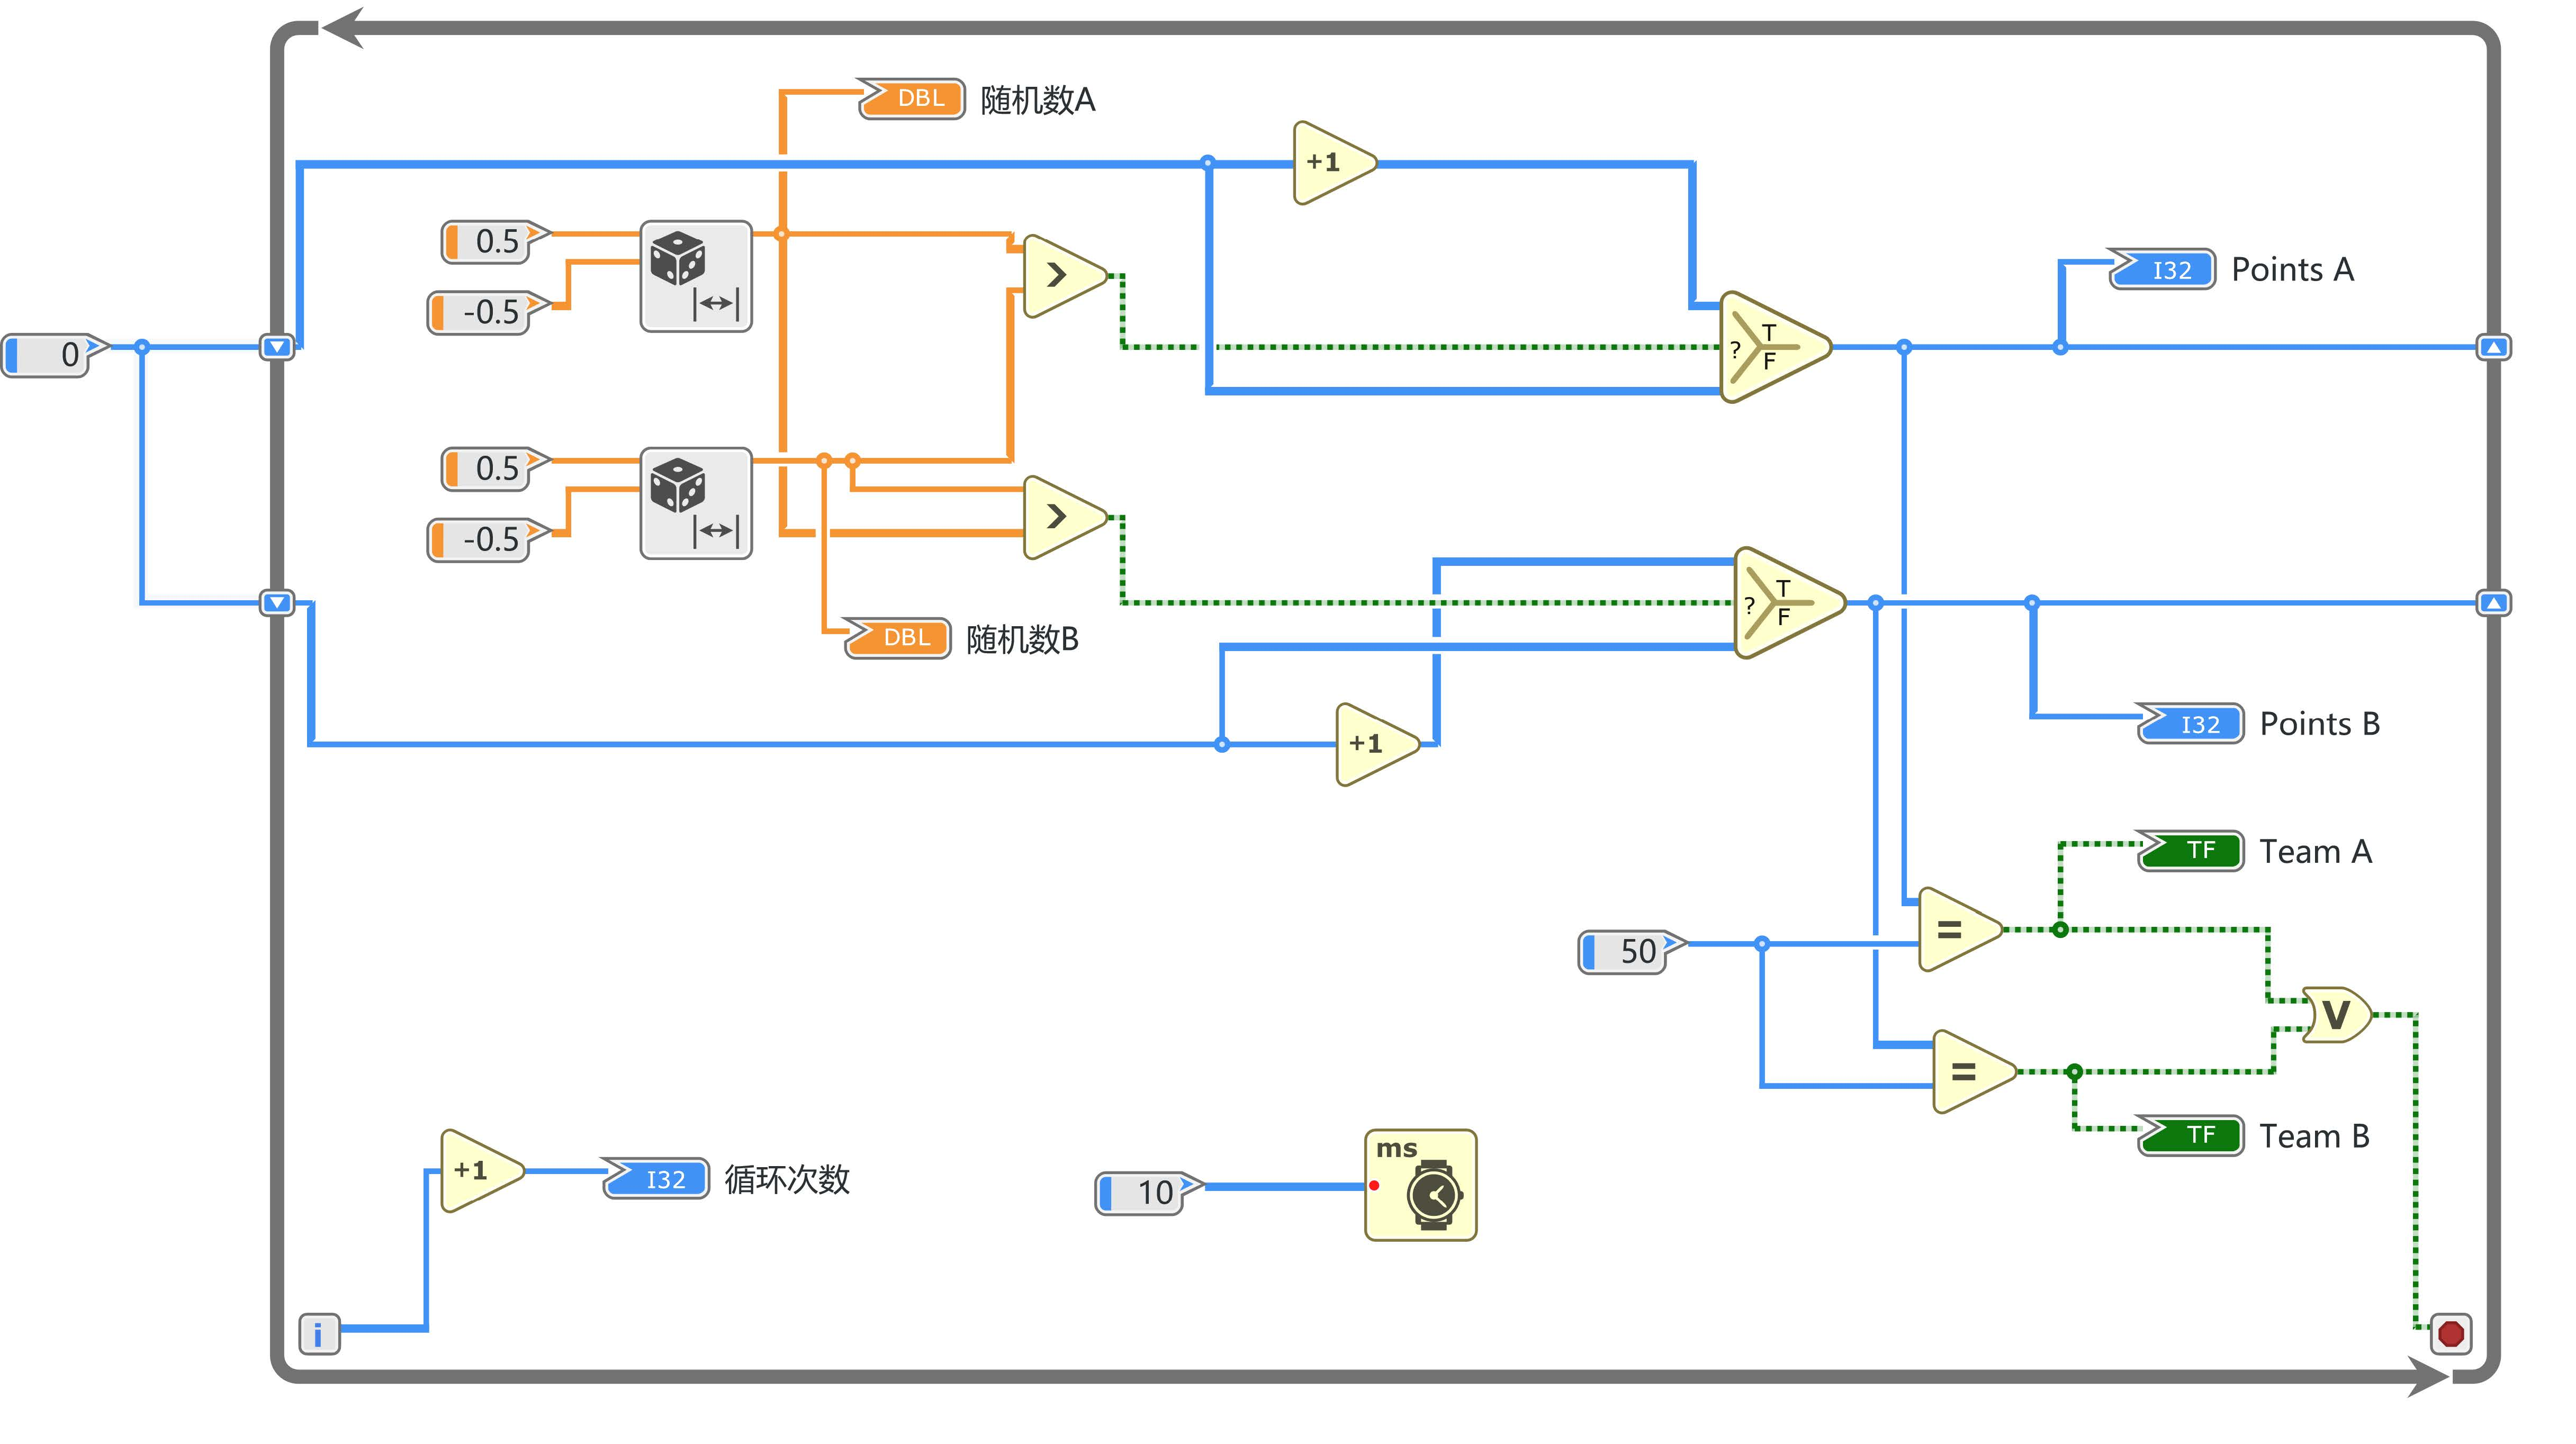
\includegraphics[width = 0.8\textwidth]{lab8/lab1-AB得分-a.jpg}
            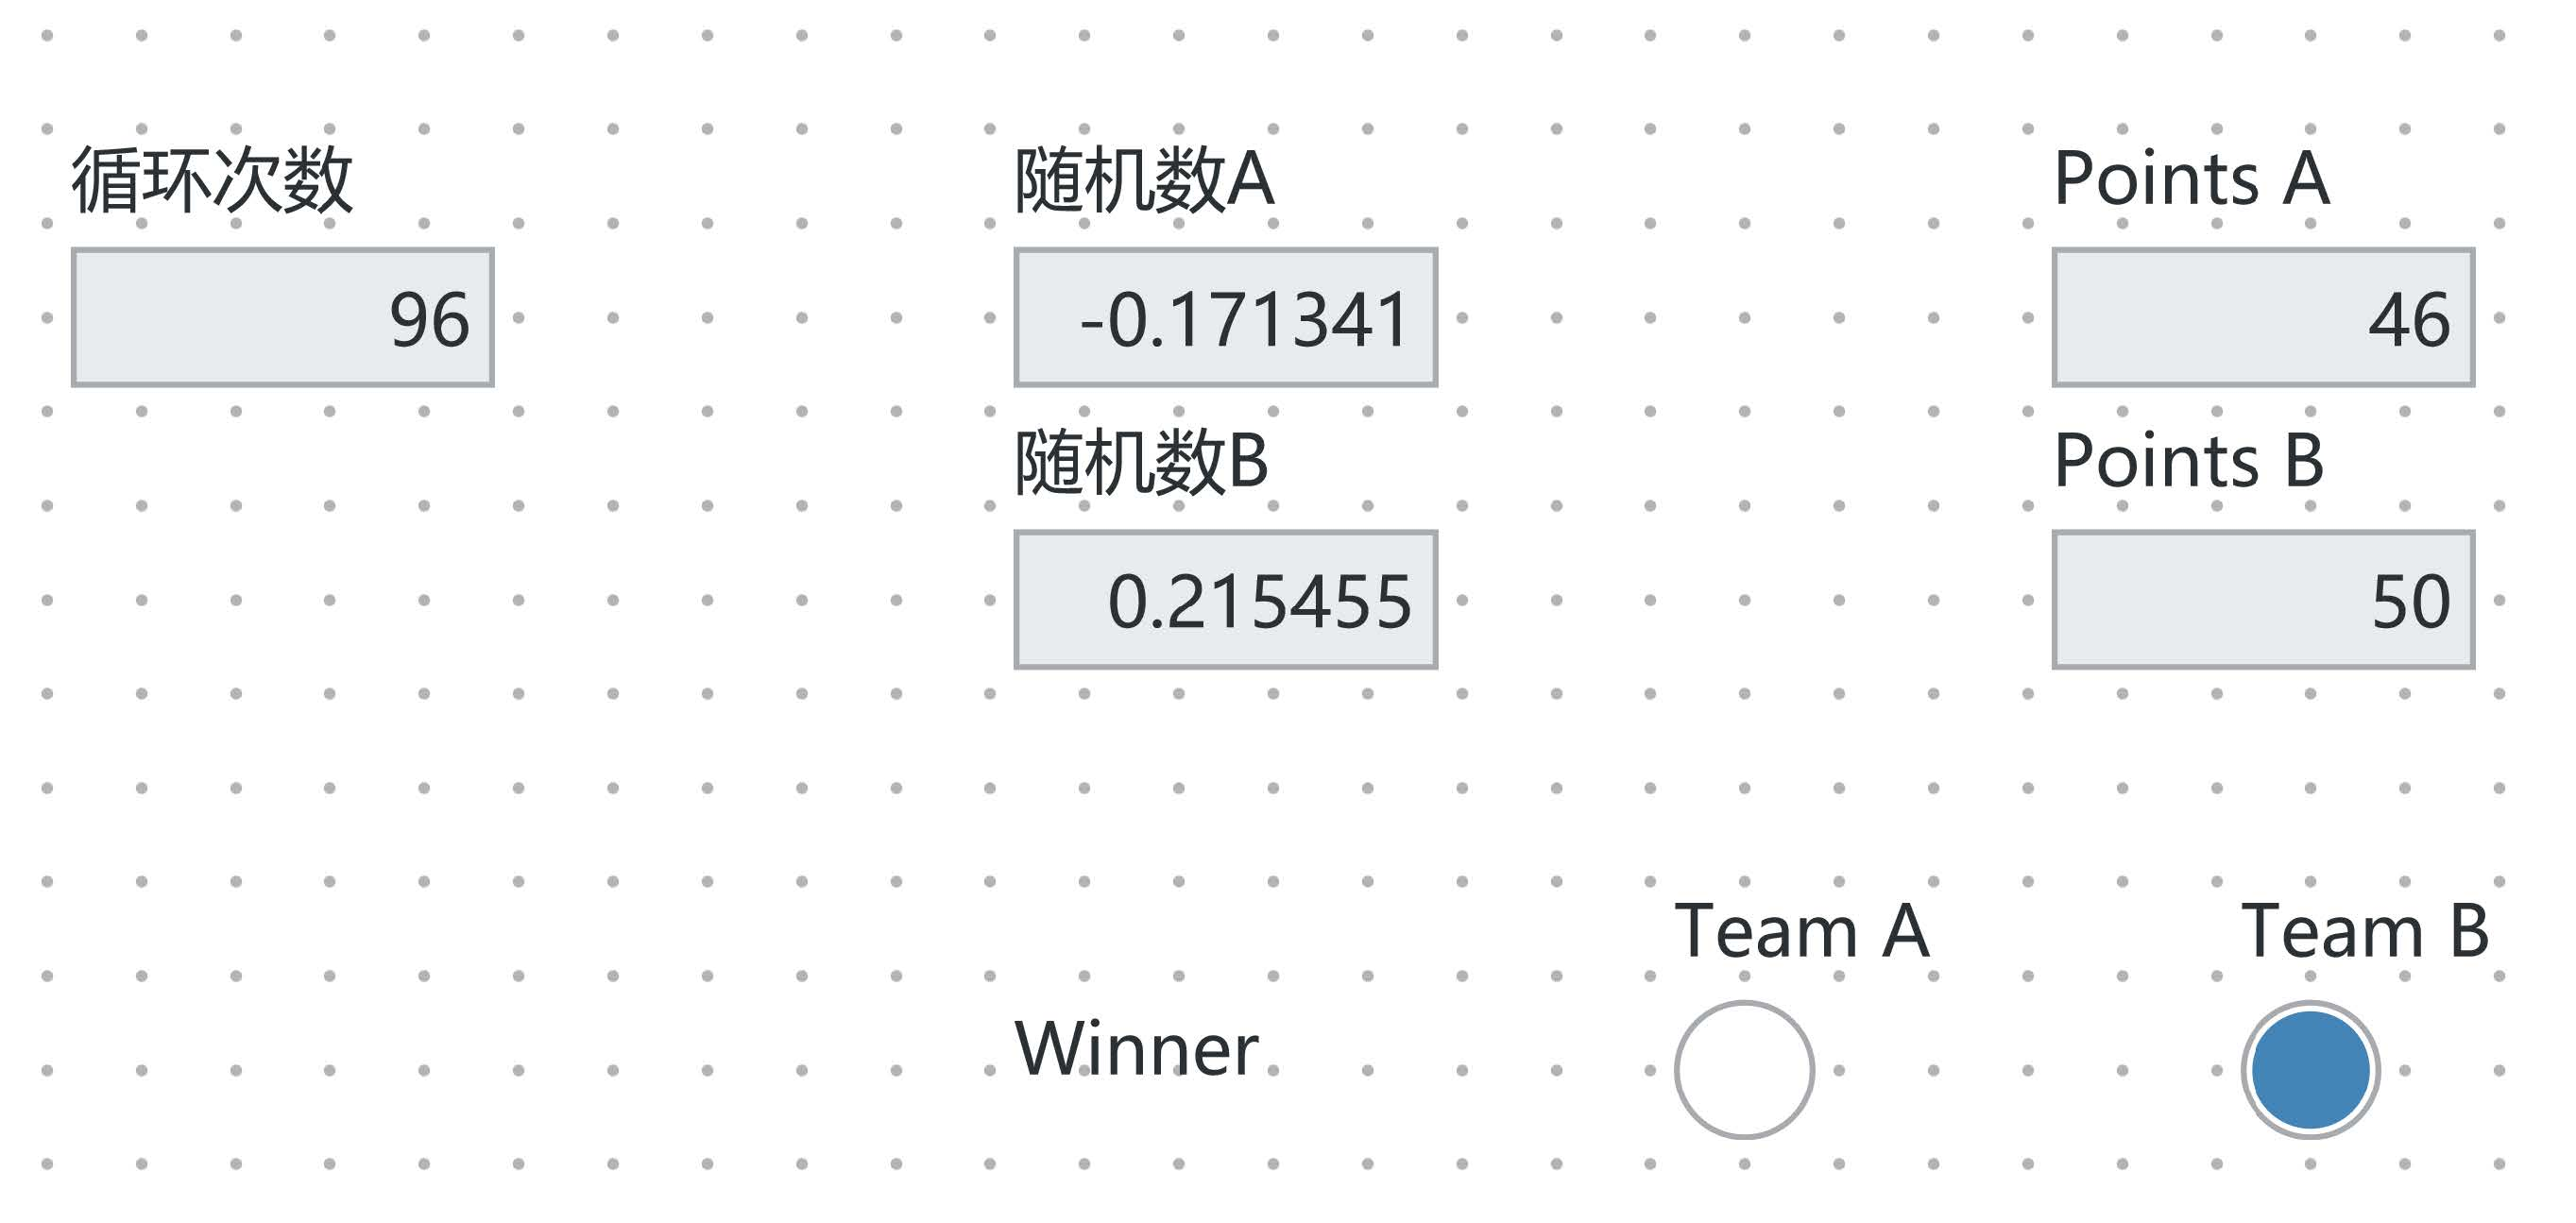
\includegraphics[width = 0.5\textwidth]{lab8/lab1-AB得分-b.jpg}
            \caption{问题4}
        \end{figure}

        

\end{document}